\documentclass[letterpaper,12pt,oneside]{book}
\usepackage[utf8]{inputenc}
\usepackage[table]{xcolor}
\usepackage[spanish]{babel}
\usepackage{amsmath}
\usepackage{amsfonts}
\usepackage{amssymb}
\usepackage{svg}
\usepackage{slashbox}
\usepackage[top=1.5cm, right=1.5cm, left=3cm, bottom=2cm]{geometry}
\usepackage{setspace}
\pagestyle{plain}
\spanishdecimal{.}


\usepackage{graphicx}

\begin{document}
	
	\begin{titlepage}

		
		\begin{center}
			
			\noindent
			\hspace{-0.1\textwidth}\rule{1.1\textwidth}{4px}\vspace{-0.08cm}
			
			\hspace{-0.1\textwidth}\rule{1.1\textwidth}{8px}\vspace{-0.23cm}
			
			\hspace{-0.1\textwidth}\rule{1.1\textwidth}{4px}
			
	
			\hspace{-0.125\textwidth}\Huge{UNIVERSIDAD DE GUADALAJARA}
			
			\hspace{-0.125\textwidth}\large{CENTRO UNIVERSITARIO DE CIENCIAS EXACTAS E INGENIERÍAS}
			
			\noindent
			\hspace{-0.1\textwidth}\rule{1.1\textwidth}{4px}\vspace{-0.2cm}
			
			\hspace{-0.1\textwidth}\rule{1.1\textwidth}{8px}\vspace{-0.33cm}
			
			\hspace{-0.1\textwidth}\rule{1.1\textwidth}{4px}
		\end{center}
		
		
		\begin{center}
			
			
			\begin{figure}[h!]
				\centering
				
\includegraphics[width=5cm]{Escudo.pdf}
			\end{figure}
		
			
		\huge{Termodinámica del oscilador armónico pateado clásico}
		
		\rule{1\textwidth}{7px}\vspace{-.8cm}
		\rule{1\textwidth}{3px}
		
		\Huge\textbf{TESIS}
		
		\hbox spread 0.4\linewidth{\Large{QUE PARA OBTENER EL TÍTULO DE}}
		
		
		
		\Huge\textbf{LICENCIADO EN FÍSICA}
		
		\hbox spread 0.75\linewidth{\Large{P R E S E N T A}}
		
		
		\Huge\textbf{{HUGO ALEXIS TORRES PASILLAS}}
		
		\huge{\textbf{Director: }Dr. Thomas Gorin}
			
		\rule{1\textwidth}{7px}\vspace{-.75cm}
		\rule{1\textwidth}{3px}
		
		\end{center}
	
	\begin{flushright}
		\Large{INVIERNO, 2020}
	\end{flushright}
\vspace{-1.7cm}
	\begin{flushleft}
		\Large{Guadalajara, Jal. Méx}
	\end{flushleft}
		
	\end{titlepage}
	\renewcommand{\baselinestretch}{2}
	\pagenumbering{Roman}
	\doublespacing
	\begin{flushright}
		
		\large{\emph{Dedicatoria}}
	\thispagestyle{empty}
	\end{flushright}
	\newpage
	\thispagestyle{empty}

		{\huge \textbf{AGRADECIMIENTOS}}
		
	
	\newpage
	
	\chapter*{Resumen}
	
	Consideramos un sistema estadístico compuesto por partículas en un potencial de oscilador
	armónico acoplado a un reservorio térmico, sujeto a patadas periódicas. Mediante el uso de las
	ecuaciones clásicas se obtienen las trayectorias en el espacio de fase, primero suponiendo que la
	temperatura del reservorio es cero, y posteriormente considerando una temperatura mayor utilizando la ecuación de Langevin. Típicamente se estudian colecciones de trayectorias, lo cual permite
	considerar la función de distribución en el espacio de fase. El comportamiento de esta función
	es similar a su equivalente cuántico. Una vez que el sistema alcanza el cuasi-equilibrio, donde la
	energía disipada por el sistema en forma de calor es igual a la recibida por las patadas, se estudia	la validez de la ley de Fourier para el sistema. Se comparan las distribuciones de las trayectorias de	las partículas en el cuasi-equilibrio con las distribuciones de Boltzmann. Finalmente, se estudian 2 ciclos termodinámicos y se compararan con los del oscilador sin patadas.
	

	\tableofcontents
	\newpage
	\listoffigures
	\newpage
	
	\newpage
	\setcounter{page}{1}
	\pagenumbering{arabic}
	
	\chapter{Introducción}
		El oscilador armónico pateado es un sistema que ha sido estudiado anteriormente por varios autores en distintos regímenes. La dinámica de este sistema resulta de gran interés por varias razones: por un lado, su dinámica presenta islas de integrabilidad en el espacio de fase para ciertos parámetros, rodeadas por zonas en las que la dinámica es caótica \cite{1991ProblemChaos}. Por otro, debido a la posibilidad de realizarse de manera experimental mediante una trampa armónica de átomos que interaccionan con l\'aseres, en el que resulta posible controlar los parámetros del sistema\cite{2012Experimental}. Además, es uno de los pocos sistemas caóticos o mixtos (el único hasta donde conocemos), donde se tiene una ecuación maestra para describir el acoplamiento del sistema a un reservorio térmico, y esto no solo en el caso clásico sino también para el sistema cuántico \cite{2017Prado}.
		
		El objetivo de estudio de este sistema ha sido variado: en el régimen clásico, su enfoque principal ha sido el estudio de su espacio de fase y las islas de integrabilidad que presenta \cite{2019dynamics, 2008StabilityChaos}, mientras que en el r\'egimen cu\'antico su estudio ha sido m\'as variado, estudiando el sistema como un ejemplo de caos, su comportamiento al ser acoplado con un reservorio t\'ermico, el entrelazamiento entre los estados del sistema, entre otros \cite{1991ProblemChaos, 2017Prado, 2016Entanglement}. As\'i mismo, este sistema ha sido utilizado para el estudio de la transici\'on entre el r\'egimen cl\'asico y el cu\'antico, debido a que es posible modificar la constante efectiva de Planck $h_{\rm eff}$, mediante la modificaci\'on del par\'ametro de Lamb-Dicke \cite{2004Transition}. E incluso se han realizado estudios experimentales del sistema \cite{1991ProblemChaos, 2017Prado}.
		
		En 2003, Robert F. Mudde and all. realizaron un estudio de los osciladores arm\'onicos pateados formados al poner borbujas en el fondo de un tubo en U lleno de agua, enfocandose en las trayectorias que se formaban en su espacio de fase y el efecto de la fuerza de amortiguamiento. M\'as recientemente, en 2017 Miguel A. P. Reynoso et al. presentaron un art\'iculo en el que estudian el sistema cu\'antico acoplado a un baño t\'ermico, en diferentes reg\'imenes entre la integrabilidad del sistema y el caos, concluyendo que la energ\'ia del sistema estaba regido por la ley de Fourier en los estados estacionarios. As\'i, surgen las siguientes dudas: ¿c\'omo podr\'ia hacerse una descripci\'on termodin\'amica del sistema cl\'asico an\'alogo al presentado en \cite{2017Prado}? y ¿qu\'e similitudes habr\'ia entre ambos sistemas?
		
		El principal objetivo de este trabajo es estudiar el sistema clásico análogo al sistema cuántico estudiado en \cite{2017Prado}. De los dos efectos del entorno (disipación y difusión), comenzamos despreciando el segundo término, lo que de cierta forma es equivalente a un sistema en contacto con un entorno a temperatura cero, para obtener el efecto de la fuerza de amortiguamiento en el espacio de fase del sistema. Posteriormente, consideramos también la temperatura del reservorio resolviendo la ecuación de Langevin, donde se agrega una fuerza aleatoria que modifica las trayectorias de las partículas, generando un movimiento browniano \cite{1998LangevinEquation}.
		
		Debido al acoplamiento del sistema con el reservorio térmico, cada trayectorias del sistema se vuelve aleatoria, por lo que consideramos una colectividad con muchas trayectorias y estudiamos la estadística sobre esta. Por un lado podemos pensar en un gran número de átomos, todos siguiendo su propia trayectoria en el espacio de fase. Así, en un tiempo dado se tiene una distribución de puntos, la cual se puede describir con la función de distribución. Por otro lado podemos pensar en un solo sistema y la probabilidad de encontrarlo en un tiempo dado en cierto lugar del espacio de fase. Antes y después de cada patada, se encuentra esta función de distribución y se comparan con su equivalente en el régimen cuántico, las funciones de Wigner.
		
		Al obtener la función de distribución antes y después de cada patada, presentamos la evolución de la energía promedio de las partículas durante las patadas, la cual llega a un estado estacionario donde la energía disipada al reservorio en forma de calor es la misma que la energía suministrada por las patadas. En estos estados estacionarios estudiamos si el intercambio de calor entre el sistema y el entorno cumple o no la ley de Fourier.
		
		A continuación, comparamos la función de distribución antes y después de las patadas con las correspondientes distribuciones de Boltzmann analíticas para el oscilador arm\'onico, utilizando la divergencia de Kullback-Leibler (entre otros) para cuantificar las diferencias.
		
		Finalmente, realizamos dos ciclos termodinámicos en los que utilizamos procesos con y sin patadas, con el que comparamos los procesos isotérmicos y adiabáticos del oscilador armónico con el sistema con patadas.
	\chapter{Preliminares}
	
	A continuaci\'on, introduciremos algunos de los conceptos utilizados durante este trabajo, siguiendo el libro ``\emph{Classical Mechanics}'' de Jhon R. Taylor .......
	
	\section{Mec\'anica hamiltoniana}
	
	En la mec\'anica Lagrangiana, las ecuaciones de movimiento surgen del Lagrangiano, $L(q, \dot{q})$, que depende de las posiciones generalizadas $q$, de las velocidades generalizadas $\dot{q}$, y quiz\'a del tiempo $t$, y corresponde a la energ\'ia cin\'etica $T$ menos la ener\'ia potencial $U$:
	
	\begin{equation}
	L(q, \dot{q}, t) = T - U.
	\end{equation}
	
	Utilizando los momentos generalizados, dados por
	
	\begin{equation}
		p_i = \frac{\partial L}{\partial \dot{q}},
	\end{equation}
	
	\noindent se obtiene el Hamiltoniano, que es la funci\'on central en la formulaci\'on hamiltoniana, y est\'a dado por:
	
	\begin{equation}
		H(p, q, t) = \sum_{i=1}^n p_iq_i - L,
	\end{equation}
	
	\noindent el cual para varios sistemas corresponde a la energ\'ia total:
	
	\begin{equation}
		H(p, q, t) = T + U.
	\end{equation}
		
	Las ecuaciones de movimiento del sistema se derivan de su hamiltoniano mediante las llamadas ecuaciones de Hamilton:
	
	\begin{equation}\label{eq:HamiltonEquation}
		\dot{q_i} = \frac{\partial H}{\partial p_i} \verb|     y     | \dot{p_i} = -\frac{\partial H}{\partial q_i}.
	\end{equation}
		
	\section{Termodin\'amica}
	
	Un sistema termodin\'amico consiste en una cantidad de materia suficientemente grande (en el sentido de que la cantidad de materia usualmente se cuenta en moles), delimitado por una superfice que separa al sistema de su ambiente o alrededores, que puede ser f\'isica o imaginaria.
	
	Dependiendo del tipo de barrera que separe al sistema termodin\'amico de su alrededor, un sistema puede ser:
	
	\begin{itemize}
		\item \textbf{abierto}, si existe intercambio de materia entre el sistema y el ambiente
		
		\item \textbf{cerrado}, si la barrera no permite intercambio de materia con el ambiente
		
		\item \textbf{adiab\'atico}, si no se permite conductividad de calor con el ambiente
		
		\item \textbf{aislado}, si no se permite ninguna interacci\'on entre el sistem y el ambiente.
	\end{itemize}

	El estado de un sistema termodin\'amico est\'a descrito por un conjunto de variables termodin\'amicas, y est\'a completamente descrito por ellas, adem\'as no depende del estado pasado del sistema. Estas variables se escriben como,
	
	\begin{equation}
		{X_1, X_2, X_3, ... }.
	\end{equation}
	
	Una funci\'on de estado es una propiedad f\'isica que depende solo del estado del sistema, y se expresa por, 
	
	\begin{equation}
		F(X_1, X_2, X_3, ...).
	\end{equation}
	
	La termodin\'amica de un sistema obedece a las siguientes leyes, conocidas como leyes de la termodin\'amica:
	
	\begin{itemize}
		\item \textbf{Ley cero.} Si dos sistemas A y B se encuentran en equilibrio termodin\'amico con un tercer sistema C, entonces A y B se encuentran en equilibrio termodin\'amico entre s\'i, lo que permite definir una funci\'on de temperatura emp\'irica.
		
		\item \textbf{Primera ley (conservaci\'on de la energ\'ia).} Para cada sistema, existe una variable termodin\'amica escalar extensiva llamada energ\'ia (U). Para el caso de un sistema cerrado, 
		
		\begin{equation}
			dU = \delta W + \delta Q, 
		\end{equation}
		
		\noindent donde $\delta U$ y $\delta Q$ son el diferencial del trabajo y el calor, respectivamente, en los que se utiliza el s\'imbolo $\delta$ para representar que no son diferenciales exactos.
		
		\item \textbf{Segunda ley. } No existe un proceso c\'iclico que tenga el \'unico efecto de transferencia de calor de un cuerpo a temperatura $T_1$ a otro de temperatura $T_2$, si $T_1 < T_2$. Lo que implica adem\'as que existe una variable termodin\'amica llamada entrop\'ia, denotada por $S$, y que en cualquier proceso termodin\'amico $ \frac{\delta Q}{T} \leq dS$, donde T es un denominador integrante del calor. 
	\end{itemize}
	
	\section{Colectividad can\'onica}
	
	En la colectividad can\'onica se considera un sistema en contacto con un baño t\'ermico a una temperatura controlada $T$, de manera que el sistema se encuentra en equilibrio termodin\'amico con sus fronteras a una temperatura tambi\'en $T$. 
	
	La funci\'on de distribuci\'on del sistema, que nos da la probabilidad de encontrar a una part\'icula de este en el estado $(\vec{p},\vec{q})$ del espacio de fase, donde $\vec{p}$ y $\vec{q}$  son las posiciones y los momentos generalizados del sistema, respectivamente, est\'a dada por:
	
	\begin{equation}
		\rho = \frac{1}{\Omega(T, \vec{X})} e^{\frac{H(\vec{p}, \vec{q})}{k_B T}},
	\end{equation}
	
	\noindent donde $H(\vec{p}, \vec{q})$ es el hamiltoniano del sistema y  $k_B$ es la constante de Boltzmann. La funci\'on $\Omega(T, \vec{X})$ es la constante de normalizaci\'on de la funci\'on de distribuci\'on llamada funci\'on de partici\'on de la colectividad can\'onica, que depende de la temperatura del reservorio T y las las variables mec\'anicas del sistema, y est\'a dada por
	
	\begin{equation}
		\Omega(T, \vec{X}) = \int \frac{dp_1 dp_2 ... dq_1 dq_2...}{h^NN!} e^{\beta H(\vec{p}, \vec{q})}, 
	\end{equation}
	
	\noindent donde N es el n\'umero de part\'iculas que componen al sistema termodin\'amico y $\beta = \frac{1}{k_BT}$.
	
	Las propiedades termodin\'amicas se pueden deducir a partir de esta funci\'on de partici\'on:
	
	\begin{itemize}
		\item Energ\'ia interna
		
		\begin{equation}
			U = -\frac{\partial}{\partial \beta} ln\Omega(T, \vec(X)).
		\end{equation}
		
		\item Diferencial de trabajo
		
		\begin{equation}
			\delta W = \frac{1}{\beta}\sum_{\alpha=1}^K\frac{\partial}{\partial X_{\alpha}}ln\Omega(T, \vec{X})dX_\alpha.
		\end{equation}
		
		\item Entrop\'ia
		
		\begin{equation}
			S = \frac{U}{T} + k_Bln\Omega(T, \vec{X})
		\end{equation}
	\end{itemize}	
	
	%\section{El oscilador arm\'onico pateado}
	
	\chapter{Marco te\'orico}
	
	El oscilador arm\'onico pateado es un sistema f\'isico cuya din\'amica est\'a descrita por el Hamiltoniano siguiente:
	
	\begin{equation}\label{Hamiltoniano}
		H = \omega \hbar \left[ \frac{p^2}{2} + \frac{x^2}{2} \right] + \frac{\kappa}{\sqrt{2}\eta^2} \cos \left( \sqrt{\frac{2\hbar}{m\omega}}\eta x  \right) \sum_{n\in\Re}\delta(t/\omega - n\tau_k),
	\end{equation}
	
	\noindent donde se han tomado los par\'ametros para la posici\'on, el momento y el tiempo como 
	
	\begin{equation}\label{CambioVariables}
		x = \sqrt{\frac{m\omega}{\hbar}}X, \verb|    | p = \frac{P}{\sqrt{\hbar m \omega}}, \verb|    | \tau = \omega t,
	\end{equation}
	
	\noindent siendo $X$ y $P$ la posici\'on y el momento de la part\'icula en unidades f\'isicas respectivamente, $m$ su masa y $\omega$ la frecuencia del oscilador. El t\'ermino $\kappa$ es la llamada \textit{fuerza de la patada adimensional}, $\eta$ es el par\'ametro de Lamb-Dicke, y $\tau_k$ el periodo en el que act\'ua la patada, cuyo potencial corresponde al tercer t\'ermino del hamiltoniano. $\hbar$ es la constante de Planck y $\delta$ es la delta de Dirac.
	
	\section{Din\'amica en el espacio de fase}
	
	Las trayectorias en el espacio de fase de este sistema corresponden a las del oscilador arm\'onico, mientras que durante el efecto de las patadas, cada tiempo $t = n\tau_k$, las part\'iculas cambian instant\'aneamente su momento pero mantienen la misma posici\'on, cambiando a otra trayectoria del oscilador arm\'onico de energ\'ia distinta.
	
	Sin embargo, al considerar el sistema acoplado a un reservorio t\'ermico ya no esposible encontrar las ecuaciones de movimiento mediante un hamiltoniano, debido al intercambio de energ\'ia del sistema con el reservorio. En su lugar, encontramos las trayectorias resolviendo la ecuaci\'on de Langevin, dada por: 
	
	\begin{equation}\label{LangevinOriginal}
		\frac{d^2x}{dt^2} + \frac{\gamma}{m}\frac{dx}{dt} + \omega^2 x = \frac{1}{m}\eta_T,
	\end{equation}
	
	\noindent donde $\gamma$ es el coeficiente de acoplamiento entre el sistema y el reservorio, y $\eta_T$ es una fuerza aleatoria que act\'ua sobre la part\'icula debido a la temperatura del entorno  con una distribuci\'on normal, provocando un movimiento browniano, dada por:
	
	\begin{equation}\label{EtaTemperatura}
		\langle \eta_T(t)\eta_T(t') \rangle = 2\gamma k_B T_e\delta(t-t'),
	\end{equation}
	
	\noindent donde $k_B$ es la constante de Boltzmann, $T_e$ es la temperatura del reservorio, y el t\'ermino $\delta(t-t')$ indica que la fuerza aleatoria se supone independiente para cada tiempo. 
	
	Al tomar las variables en (\ref{CambioVariables}), la ecuaci\'on de Langevin (\ref{LangevinOriginal}) queda escrita como:
	
	\begin{equation}\label{Langevin}
		\frac{d^2x}{d\tau^2} + \frac{\gamma}{m\omega}\frac{dx}{d\tau} + x = \frac{1}{\omega}\sqrt{\frac{1}{m\omega\hbar}}\eta_T.
	\end{equation} 
	
	Durante el efecto de las patadas podemos despreciar el efecto del reservorio t\'ermico durante un intervalo de tiempo arbitrariamente pequeño, debido a que la fuerza es instat\'anea, por lo que el efecto de las patadas se puede encontrar a partir del hamiltoniano del sistema original de la ecuaci\'on (\ref{Hamiltoniano}).
	
	
	Consideramos una colecci\'on estad\'istica de trayectorias, de forma que en cada instante de tiempo $t$ estas nos dan una distribuci\'on de estados en el espacio de fase correspondiente a la funci\'on de distribuci\'on del sistema, que corresponde a una densidad de probabilidad de encontrar una parti\'icula en cierto lugar del espacio de fase, la cual se vuelve cuasi-estacionaria para tiempos suficientemente grandes. Esta funci\'on de distribuci\'on se compara con su equivalente cu\'antico.
	
	\subsection{Soluci\'on a la ecuaci\'on de Langevin}
	
	Para encontrar la soluci\'on de la ecuaci\'on de Langevin en (\ref{Langevin}), comenzamos escribiendo dicha ecuaci\'on diferencial como un sistema de ecuaciones de primer orden:
	
	\begin{equation}
		\begin{bmatrix}
		x \\ p
		\end{bmatrix}' = 
		\begin{bmatrix}
		0 & 1 \\
		-1 & -\frac{\gamma}{m\omega}
		\end{bmatrix}
		\begin{bmatrix}
		x \\ p
		\end{bmatrix} 
		+
		\begin{bmatrix}
		0 \\ \eta_T\frac{1}{\omega}\sqrt{\frac{1}{m\omega\hbar}}
		\end{bmatrix}.
	\end{equation}
	
	
	
	 El t\'ermino $\eta_T$ de la fuerza aleatoria debido a la temperatura se obtiene a partir de la ecuaci\'on (\ref{EtaTemperatura}). Introduciendo la variable aleatoria $x_j$ con distribuci\'on normal y varianza $\langle x_j^2 \rangle = 1$, podemos escribir dicha ecuaci\'on como
	
	\begin{equation}
		\langle \eta_T(t)x(t)\eta_T(t^{'})x(t^{'}) \rangle = 2\gamma k_BT_e\delta(t-t^{'
		}),
	\end{equation}
	
	\noindent integrando en ambos lados, obtenemos:
	
	\begin{equation}
		\eta_T^2x_j^2\Delta t = 2\gamma k_B T.
	\end{equation}
	
	Por lo tanto, el t\'ermino de la patada aleatoria es
	
	\begin{equation}\label{EtaTemperaturaCalculado}
		\eta_T^2 = \frac{2\gamma k_BT}{\Delta \tau}.
	\end{equation}
	
	Utilizando el m\'etodo n\'umerico de Euler-Maruyama para resolver ecuaciones diferenciales estoc\'asticas, la ecuaci\'on de Langevin puede ser resuelta por
	
	\begin{equation}
		\begin{bmatrix}
		x \\ p
		\end{bmatrix}_{n+1}' = 
		\begin{bmatrix}
		x \\ p
		\end{bmatrix}_{n}
		+ \Delta\tau
		\begin{bmatrix}
		0 & 1 \\
		-1 & -\beta
		\end{bmatrix}
		\begin{bmatrix}
		x \\ p
		\end{bmatrix}_n
		+
		\begin{bmatrix}
		0 \\ \frac{1}{\omega}\sqrt{ 2\beta\frac{k_BT}{\hbar}{\Delta t} }
		\end{bmatrix},
	\end{equation}
	
	\noindent donde se ha definido el t\'ermino $\beta = \frac{\gamma}{m\omega}$, el cual tomaremos como constante. El intervalo $\tau_k$ durante el que se resuelve esta ecuaci\'on se ha dividido en N subintervalos iguales $\Delta\tau = \tau_k / N$, y el sub\'indice en los vectores columna del punto en el espacio de fase corresponden al estado despu\'es de ese subintervalo.
	
	\subsection{Efecto de las patadas}
	
	Durante el efecto de las patadas podemos despreciar la temperatura del entorno debido a que esta fuerza es instant\'anea, por lo que utilizamos el hamiltoniano del oscilador arm\'onico pateado dado por la ecuaci\'on (\ref{Hamiltoniano}). Utilizando las ecuaciones de Hamilton para el momento, obtenemos:
	
	\begin{equation}
		\dot{p} = -\hbar\omega x + \frac{\kappa}{\eta}\sqrt{\frac{\hbar}{m\omega}}\sin \left[ \sqrt{\frac{2\hbar}{m\omega_k}} \eta x\right] \sum_n\delta(t-n\tau_k).
	\end{equation}
	
	Resolvemos esta ecuaci\'on durante el intervalo de tiempo $t=n\tau_k - \epsilon$ a $t=n\tau_k + \epsilon$ con $\epsilon$ arbitrariamente pequeño y tomamos el l\'imite $\epsilon \rightarrow 0$, con lo que obtenemos el cambio de la n-\'esima patada:
	
	\begin{equation}
		\Delta p = \frac{\kappa}{\eta}\sqrt{\frac{\hbar}{m\omega}} \sin \left(\sqrt{\frac{2\hbar}{m\omega}} \eta x \right).
	\end{equation}
	
	Por lo tanto,  el estado justo despu\'es de la patada es
	
	\begin{equation}\label{EfectoPatada}
		(x_n,\verb|  | p_n) = (x_n^{'}, \verb|  | p_n^{'} +  \frac{\kappa}{\eta}\sqrt{\frac{\hbar}{m\omega}} \sin \left(\sqrt{\frac{2\hbar}{m\omega}} \eta x \right),
	\end{equation}
	
	\noindent donde $x_n^{'}$ y $p_n^{'}$ son la posici\'on y el momento de la part\'icula justo antes de la n-\'esima patada.
	
	\subsection{Din\'amica del sistema}
	
	La figura \ref{fig.Temp0vsTempFinita} mestra una trayectoria en el espacio de fase del oscilador arm\'onico pateado, con el reservorio a temperatura cero y con el reservorio a temperatura finita, $k_BT_e = 5$.
	
	\begin{figure} 
		\centering 
		\begin{minipage}{0.45\textwidth}
			\centering 
			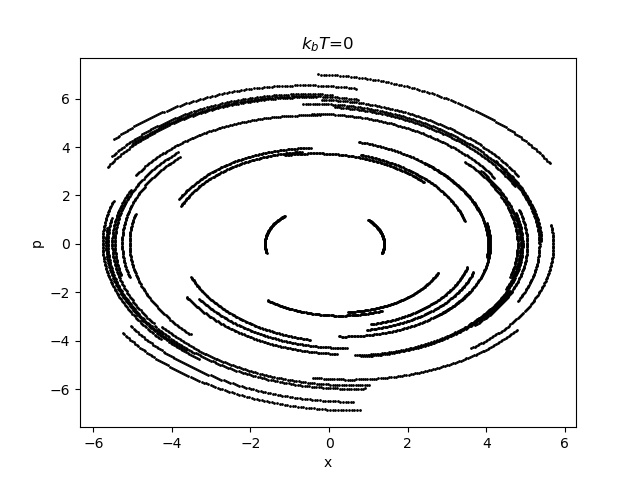
\includegraphics[width=8cm]{Figures/noT}
		\end{minipage}
		\begin{minipage}{0.45\textwidth}
			\centering 
			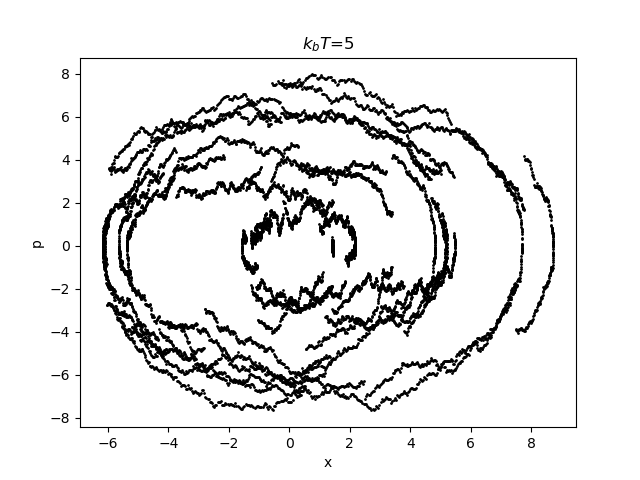
\includegraphics[width=8cm]{Figures/10T}
		\end{minipage}
		
		\caption{Trayectoria en el espacio de fase del oscilador armónico pateado con y sin temperatura del entorno.}
		\label{fig.Temp0vsTempFinita}
	\end{figure}
	
	 A partir del punto $(x_n, p_n)$ en el espacio de fase del sistema justo antes de la n\'esima patada, calculamos el estado $(x_{n+1}^{'}, p_{n+1}^{'})$ justo despu\'es de la patada $n$ utilizando la ecuaci\'on (\ref{Langevin}), y posteriormente utilizamos el hamiltoniano del oscilador arm\'onico pateado en la ecuaci\'on (\ref{Hamiltoniano}) para aplicar el efecto (instant\'aneo) de la patada, obteniendo el punto $(x_{n+1}, p_{n+1})$ en el espacio de fase, correspondiente al estado del sistema justo antes de la patada $n+1$.
	
	La dinámica del sistema queda determinado por la fuerza de las patadas $\kappa$, la relación entre las dos frecuencias del sistema $q = \frac{\omega_k}{\omega}$, donde $\omega$ es la frecuencia del oscilador y $\omega_k$ es la frecuencia de las patadas, y el coeficiente de acoplamiento del sistema con el reservorio $\beta$, mientras que el parámetro $\eta$ nos da únicamente un  re-escalamiento del espacio de fase \cite{PradoTesis} como se muestra en la figura \ref{Img:Reescalamiento}.
	
	\begin{figure}[h!]
		\centering
		\begin{minipage}{0.35\textwidth}
			\centering
			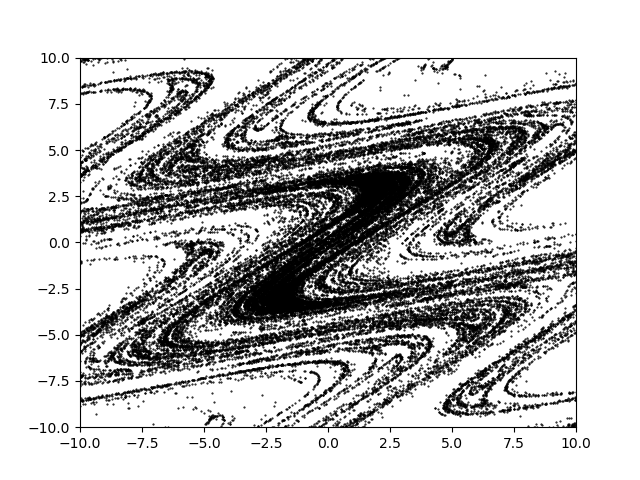
\includegraphics[width=7cm,height=5cm]{Figures/Eta05}
		\end{minipage}
		\begin{minipage}{0.35\textwidth}
			\centering
			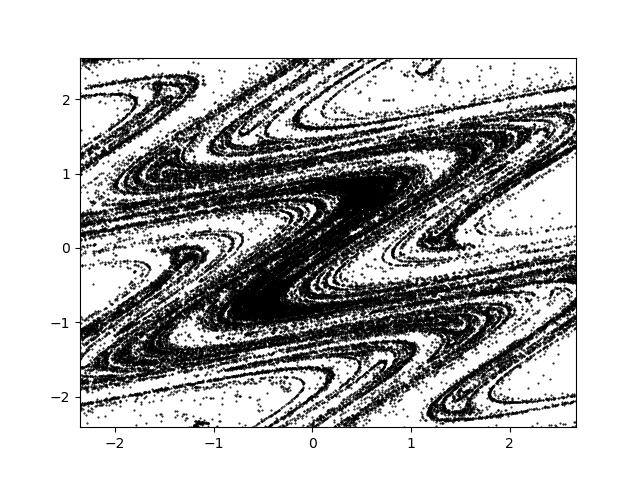
\includegraphics[width=7cm,height=5cm]{Figures/Eta20}
		\end{minipage}
		\caption{Espacio de fase para $\eta=0.5$ y $\eta=2.0$}
		\label{Img:Reescalamiento}
	\end{figure}

	\section{Interpretaci\'on termodin\'amica}
	
	A partir del mapa del espacio de fase obtenido anteriormente, podemos encontrar la energía promedio de las partículas mediante el promedio de la energía cinética y potencial de cada una de ellas en la n-ésima patada,
	
	\begin{equation}
	\langle E(n) \rangle = \frac{1}{N}\sum_{j=1}^{N} \omega(\frac{p_j^2}{2} + \frac{q_j^2}{2}),
	\end{equation}
	
	\noindent donde $p_j$ y $q_j$ son las coordenadas de posición y el momento de cada partícula.
	
	
	Y de esta forma, podemos encontrar la evolución temporal de la energía en cada patada. Sin embargo, el sistema tiene dos energías promedio en cada patada, una justo antes y la otra justo después de cada una de ellas.
	
	Si después de un número $N_e$ de patadas el sistema logra llegar a un punto de cuasi-equilibrio entre la energía disipada por el efecto del amortiguamiento y la energía suministrada por las patadas, podemos calcular el promedio de la energía del sistema antes y después de las patadas en este estado como
	
	\begin{eqnarray}
	\langle E \rangle_b &=& \frac{1}{N_k - N_e} \sum_{n = N_e}^{N_k}  \langle E_b(n)\rangle \label{Eq.MHBefore}\\ 
	\langle E \rangle_a &=& \frac{1}{N_k - N_e} \sum_{n = N_e}^{N_k}  \langle E_a(n) \rangle , \label{Eq.MHafter}
	\end{eqnarray}
	
	\noindent donde $\langle E \rangle_b$ y $ \langle E \rangle_a $ son el promedio de la energía sobre el tiempo en el estado de equilibrio antes y después de las patadas, respectivamente, $N_e$ es el número de patadas del sistema al alcanzar el cuasi-equilibrio y $N_k$ es el número total de patadas, con $N_e<N_k$, y $\langle E_b(n) \rangle$ y $\langle E_a(n) \rangle$ son las energías del sistema antes y después de la n-ésima patada, respectivamente.
	
	La energía promedio total del sistema en el cuasi-equilibrio la podemos obtener con los dos resultados anteriores como
	
	\begin{equation}\label{Eq.MeanET}
	\langle E \rangle = \frac{\langle E \rangle_b + \langle E \rangle_a}{2}.
	\end{equation}
	
	Además, podemos encontrar la cantidad de energía disipada entre dos patadas consecutivas mediante la resta del promedio de la energía del sistema antes y después de las patadas
	
	\begin{equation}\label{Eq.DeltaE}
	\Delta E = \langle E \rangle_a - \langle E \rangle_b.
	\end{equation}
	
	Para el oscilador armónico unidimensional, la relación entre la energía interna $U$ y la temperatura está dada por
	
	\begin{equation} \label{Eq.EnergiaInterna}
	U = N K_B T
	\end{equation}
	
	\noindent donde N es el número de partículas del sistema y $k_B$ es la constante de Boltzman \cite{CursoFisEstadistica}. Utilizando la energía promedio del sistema obtenida de forma numérica, la relación entre la temperatura y la energía del sistema es
	
	\begin{equation}
	\langle E \rangle = k_BT
	\end{equation}
	
	La conducción de calor entre un sistema y su entorno viene dada por la ley de Fourier
	
	\begin{equation}\label{Eq.FourierGeneral}
	\frac{Q}{t} = a(T_1 - T_2),
	\end{equation}
	
	\noindent donde $Q/t$ es el calor transmitido por unidad de tiempo, $a$ es el coeficiente de Fourier y $(T_1 - T_2)$ es la diferencia de temperatura entre la fuente caliente y fría  \cite{ModernTermo}. Consideramos la tasa de flujo de calor como la razón entre la energía disipada entre dos patadas dividida por el periodo de las patadas:
	
	\begin{equation}
	\frac{Q}{t}  = \frac{\Delta E}{\tau_k},
	\end{equation}
	
	\noindent por lo que la ley de Fourier para el sistema queda expresada como
	
	
	\begin{equation}\label{Eq.Fourier}
	\alpha \frac{\Delta E}{\tau_k} = \langle E \rangle - k_BT_e,
	\end{equation}
	
	\noindent donde $\alpha$ es el coeficiente de Fourier que nos da la constante de proporcionalidad entre ambas cantidades. El caso l\'imite del sistema aislado se obtiene al tomar $T_e = 0$.
	
	A partir de la aproximación de la energía en el oscilador armónico amortiguado \cite{Energy}, para $2\beta \ll \omega$, dada por 
	
	\begin{equation}
	E \approx \frac{1}{2}mA^2\omega^2e^{-2\beta t},
	\end{equation}
	
	
	\noindent encontramos la tasa de disipación de energía entre dos patadas consecutivas como
	
	\begin{eqnarray} \label{Coeficiente}
	\frac{\Delta E}{\tau_k} & \approx & \dot{E}\nonumber\\ 
	&\approx& -2\beta E.
	\end{eqnarray}
	
	Consideramos el flujo de energía del sistema al reservorio, por lo que utilizamos el signo positivo. Combinando las ecuaciones (\ref{Eq.Fourier}) y (\ref{Coeficiente}) obtenemos
	
	\begin{equation}
	\langle E  \rangle = \frac{1}{2\beta} \frac{\Delta E}{\tau_k}.
	\end{equation}
	
	Sin embargo, al considerar también la temperatura del entorno, debemos restar la energía de este, por lo que obtenemos, finalmente
	
	\begin{equation}
	\langle E  \rangle - k_BT_e = \frac{1}{2\beta} \frac{\Delta E}{\tau_k}.
	\end{equation}
	
	Al comparar la ecuación (\ref{Eq.Fourier}) con esta última aproximación analítica, obtenemos la siguiente expresión para los coeficientes de Fourier:
	
	\begin{equation}\label{eq:FourierNumericalCoeffs}
	\alpha = \frac{\langle E \rangle - k_B T_e}{\Delta E/\tau_k} \approx \frac{1}{\beta}.
	\end{equation}
	
	\section{Funci\'on de distribuci\'on del sistema}
	
	En un sistema termodinámico, la función de distribución que tiene el sistema corresponde a la distribución de Boltzmann:
	
	
	\begin{equation}\label{Eq:BoltzmannDist}
	P_B = Ae^{-\frac{H(x,p)}{k_BT}},
	\end{equation}
	
	\noindent donde $H(x,p)$ es el hamiltoniano del sistema y $A$ es la constante de normalización \cite{CursoFisEstadistica}. Para este sistema, consideramos el hamiltoniano del oscilador arm\'onico, 
	
	\begin{equation}
	H(x,p) = \frac{1}{2}\omega(p^2 + q^2),
	\end{equation}
	
	\noindent mientras que $k_BT = \langle E \rangle$ es la energía promedio del sistema. Por lo tanto, la distribución de Boltzmann para el sistema es:
	
	\begin{equation}
	P_B(x,p) = Ae^{\frac{\omega(p^2+q^2)}{2\langle E \rangle }}.
	\end{equation}
	
	Consideramos el error de la distribución del sistema obtenida como el porcentaje de diferencia con la distribución de Boltzmann, de manera que un $0\%$ indica que las distribuciones son completamente iguales, y un $100\%$ que son completamente distintas:
	
	\begin{equation}\label{eq:ErrorTotal}
	{\rm Err} =  \frac{|P_B(x,p) - Q(x,p)|}{P_B(x,p)} \times 100 \%,
	\end{equation}
	
	\noindent donde $Q(x,p)$ corresponde al histograma normalizado de la función de distribución del sistema, y $P_B(x,p)$ es la distribución de Boltzmann.
	
	Sin embargo, puede resultar más conveniente desde el punto de vista termodinámico comparar las distribuciones mediante la divergencia de Kullback-Leibler, para obtener una medida de similitud entre la distribución del sistema $P$ con la de Boltzmann para el oscilador armónico $Q$, dada por:
	
	
	\begin{equation}
	D_{\rm KL}(P||Q) = \sum_i P(i)\log\left(\frac{P(i)}{Q(i)}\right).
	\end{equation}
	
\chapter{Resultados}

Para lo siguiente, utilizaremos los par\'ametros del el sistema $\beta=0.1$, $\omega=1$, $k_BT_e=5$ y $q=4$ para el acoplamiento del sistema y el reservorio, la frecuencia del oscilador arm\'onico, la temperatura del reservorio, y la raz\'on entre la frecuencia del osciador con las patadas, respectivamente, a menos de que se especifiquen valores diferentes. 

\section{Espacio de fase del sistema}

En la figura \ref{Img:EspaciosDeFase} se muestran los resultados del espacio de fase para $q=4$ y distintos valores de $\kappa$, con 500 trayectorias durante un tiempo de 700s, para el sistema aislado (a, b y c), con el reservorio a temperatura cero (d, e y f), y para un entorno con $k_BT = 5$ (g, h, i).

\begin{figure}[h!]\label{EspaciosDeFase}
	
	\centering
	\begin{minipage}{0.32\textwidth}
		
		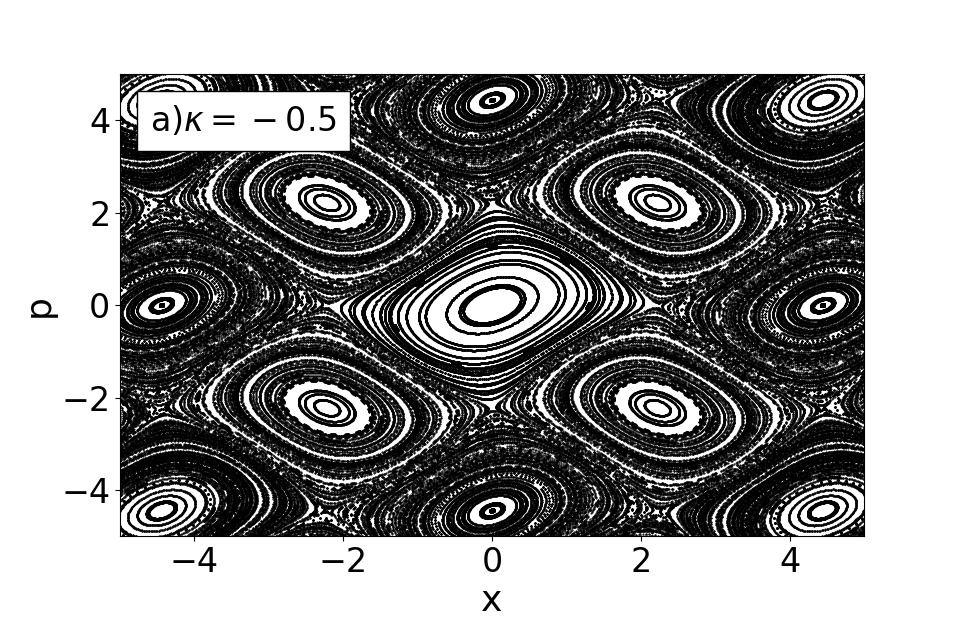
\includegraphics[width=6cm,height=4.5cm]{FigsJPG/PhaseSpace_a}
	\end{minipage}
	\begin{minipage}{0.32\textwidth}
		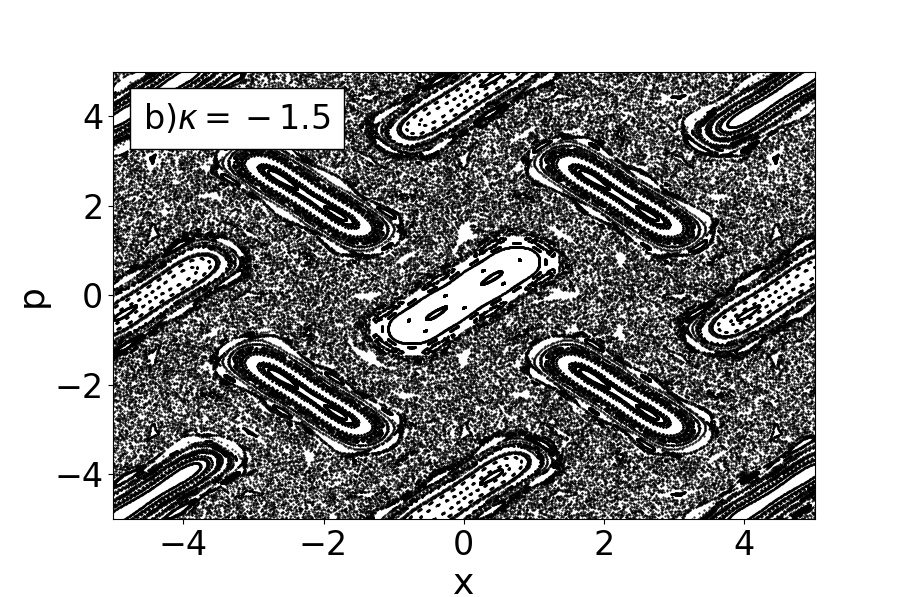
\includegraphics[width=6cm,height=4.5cm]{FigsJPG/PhaseSpace_b}
	\end{minipage}
	\begin{minipage}{0.32\textwidth}
		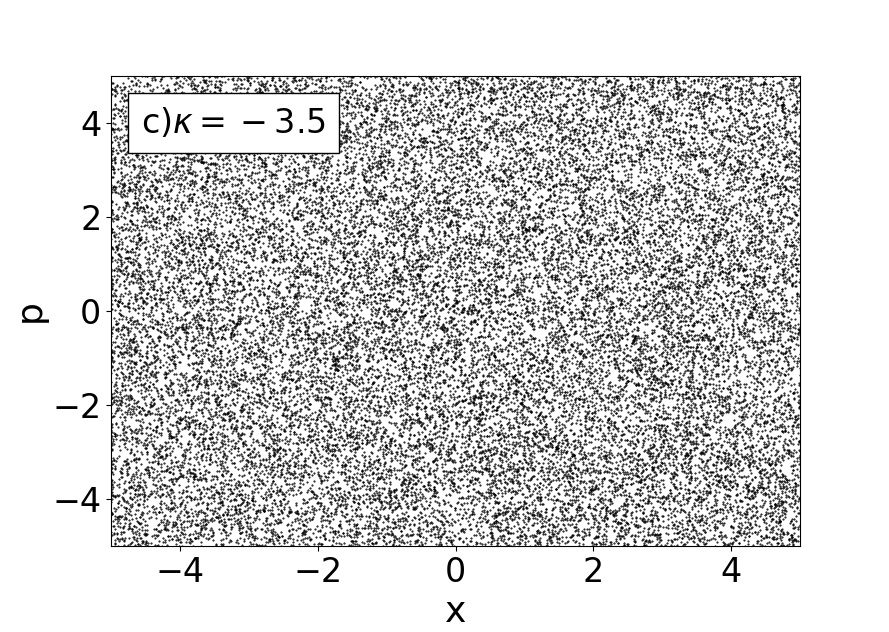
\includegraphics[width=6cm,height=4.5cm]{FigsJPG/PhaseSpace_c}
		
	\end{minipage}\\
	\begin{minipage}{0.32\textwidth}
		
		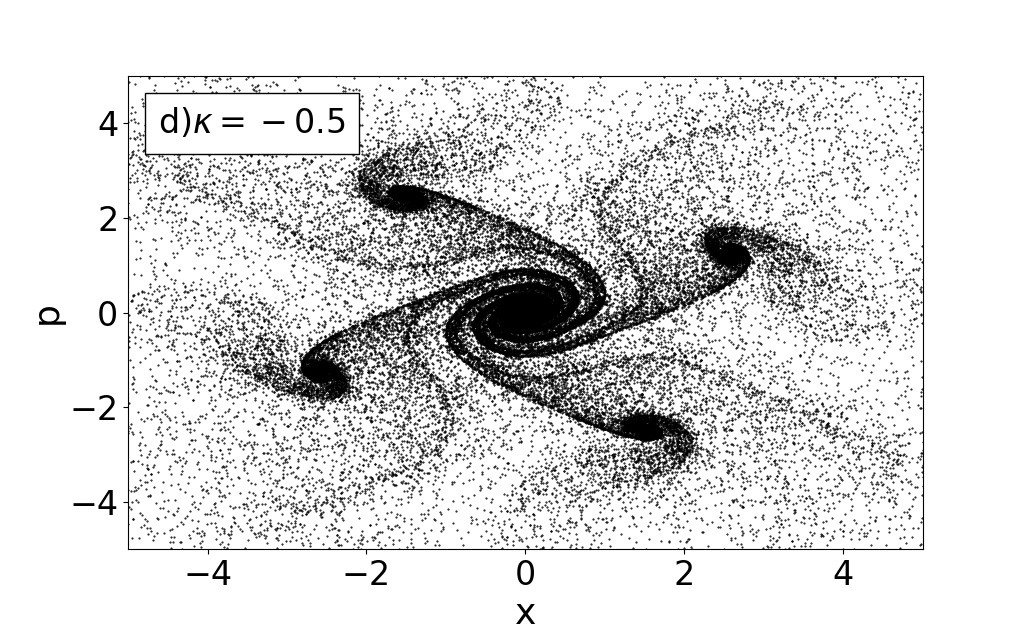
\includegraphics[width=6cm,height=4.5cm]{FigsJPG/PhaseSpace_dd}
	\end{minipage}
	\begin{minipage}{0.32\textwidth}
		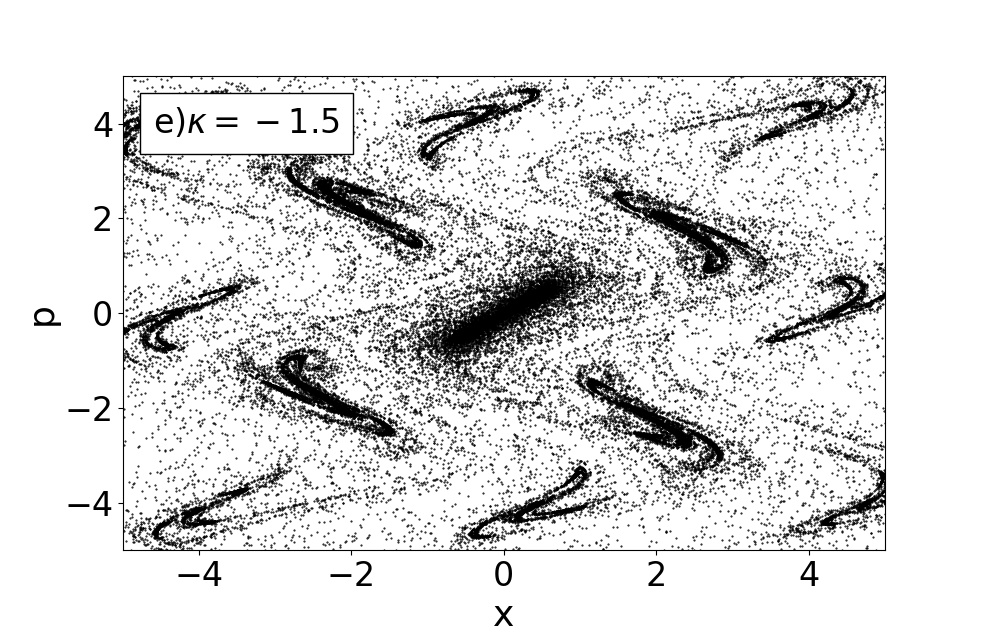
\includegraphics[width=6cm,height=4.5cm]{FigsJPG/PhaseSpace_ee}
	\end{minipage}
	\begin{minipage}{0.32\textwidth}
		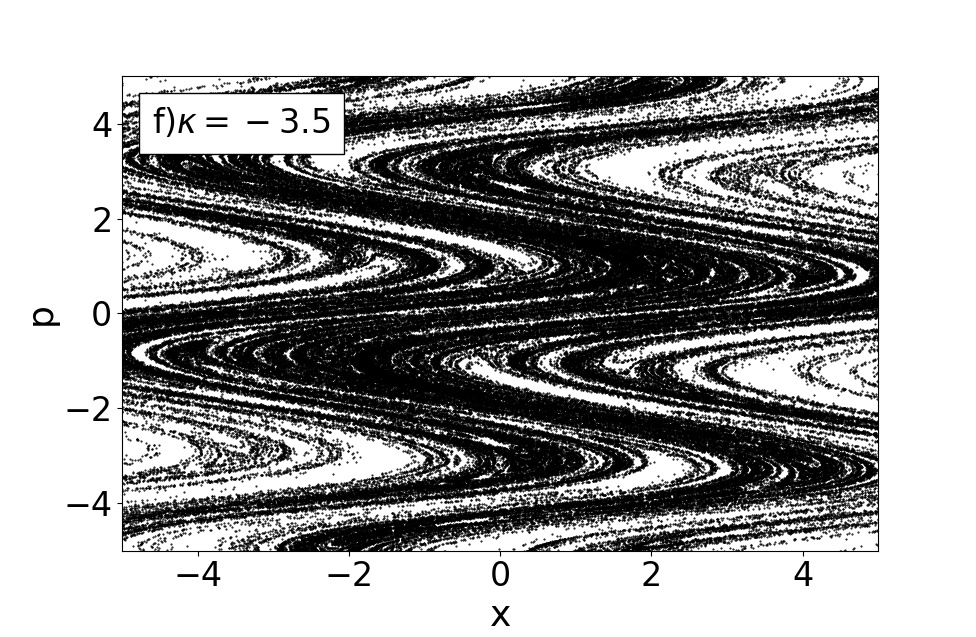
\includegraphics[width=6cm,height=4.5cm]{FigsJPG/PhaseSpace_ff}
		
	\end{minipage}\\
	\begin{minipage}{0.32\textwidth}
		
		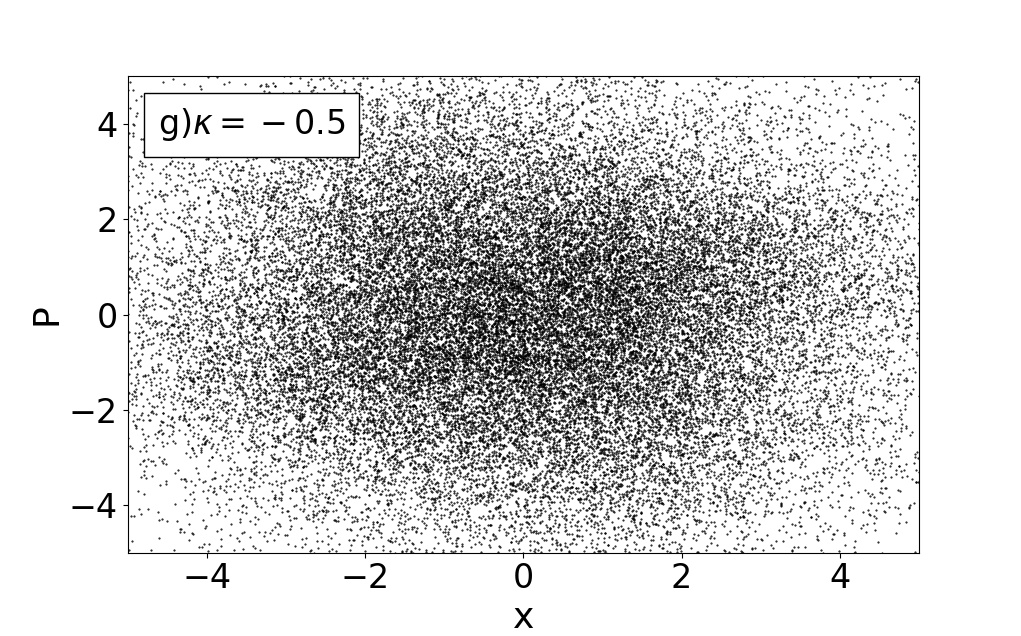
\includegraphics[width=6cm,height=4.5cm]{FigsJPG/PhaseSpace_g}
	\end{minipage}
	\begin{minipage}{0.32\textwidth}
		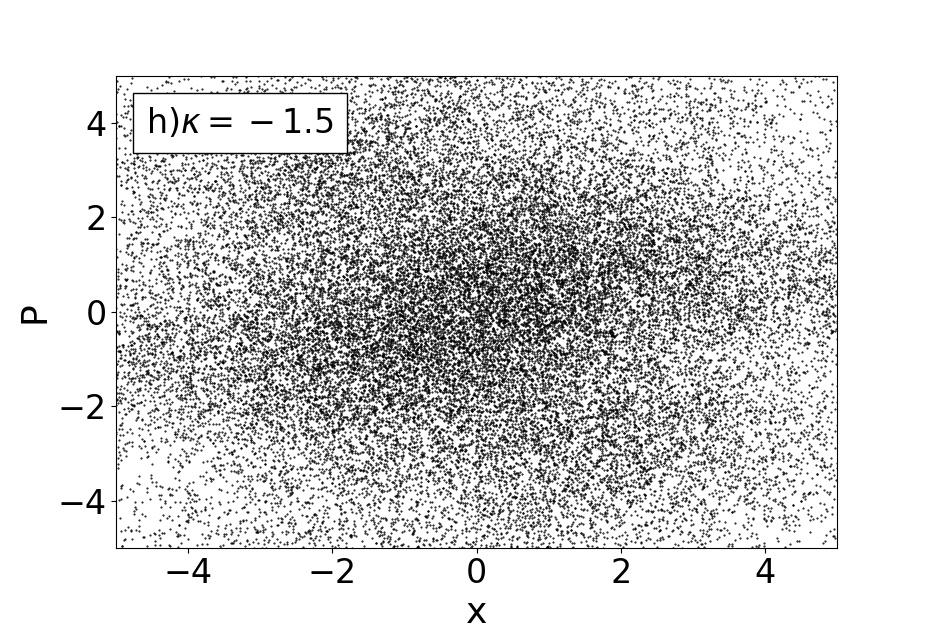
\includegraphics[width=6cm,height=4.5cm]{FigsJPG/PhaseSpace_h}
	\end{minipage}
	\begin{minipage}{0.32\textwidth}
		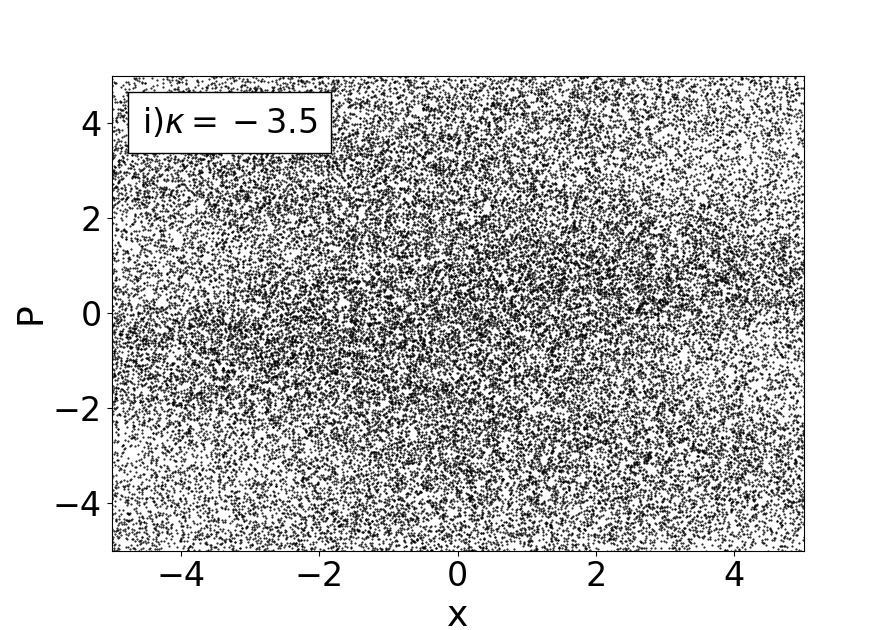
\includegraphics[width=6cm,height=4.5cm]{FigsJPG/PhaseSpace_i}
		
	\end{minipage}
	
	
	\caption{Trayectoria de 700 osciladores arm\'onicos pateados a partir de un estado inicial con distribuci\'on normal para distintos valores de $\kappa$. Las figuras a, b y c corresponden al sistema aislado y con el entorno a temperatura cero; d, e y f corresponden al sistema con el acoplamiento al reservorio y el entorno a temperatura cero; y g, h e i al sistema acoplado al reservorio con ($k_BT_e = 5$).}
	\label{Img:EspaciosDeFase}
	
\end{figure}

Para el caso del sistema aislado, $\beta=0$, donde no hay un acoplamiento con el reservorio (a, b y c en la figura \ref{Img:EspaciosDeFase}), el sistema presenta islas de integrabilidad en el espacio de fase cuando la patada es pequeña, las cuales se extienden por todo el espacio formando patrones con ciertas simetría, rodeadas por zonas caóticas que cuales se van destruyendo a medida que se aumentan las patadas pasando a tener una distribución m\'as uniforme. Sin embargo, al incluir el acoplamiento (d, e y f en las figuras \ref{Img:EspaciosDeFase}), estas islas desaparecen convirtiéndose en atractores. Para valores de $\kappa$ pequeños se mantiene una simetría similar al caso anterior. En cambio, para valores mayores de $\kappa$ el efecto del amortiguamiento domina sobre el sistema, haciendo que los estados se distribuyan de manera semejante a una oscilación, y no uniformemente como sucedía en el caso sin amortiguamiento.

Al incluir la temperatura del reservorio (g, h e i en las figura \ref{Img:EspaciosDeFase}), el sistema se vuelve completamente caótico para cualquier valor de las patadas y la distribución de las trayectorias se vuelve más uniforme.




\section{Funci\'on de distribuci\'on del sistema}

La figure {\ref{fig:DistFunctions}} muestra la funci\'on de distribuci\'on del sistema para un sistema con $\kappa=-4.5$, $k_BT_e = 5$ antes y despu\'es de la patada 1, 5 y 35 (en cada fila respectivamente). Una vez que el sistema llega al punto de quasi-equilibrio, dichas funciones se mantienen iguales antes y despu\'es de cada patada. A diferencia de las figuras mostradas en la figura \ref{Img:EspaciosDeFase}, en este caso solo se muestra el estado instant\'aneo del sistema. 

\begin{figure}[h!]
	\centering
	\label{fig:DistFunctions}
	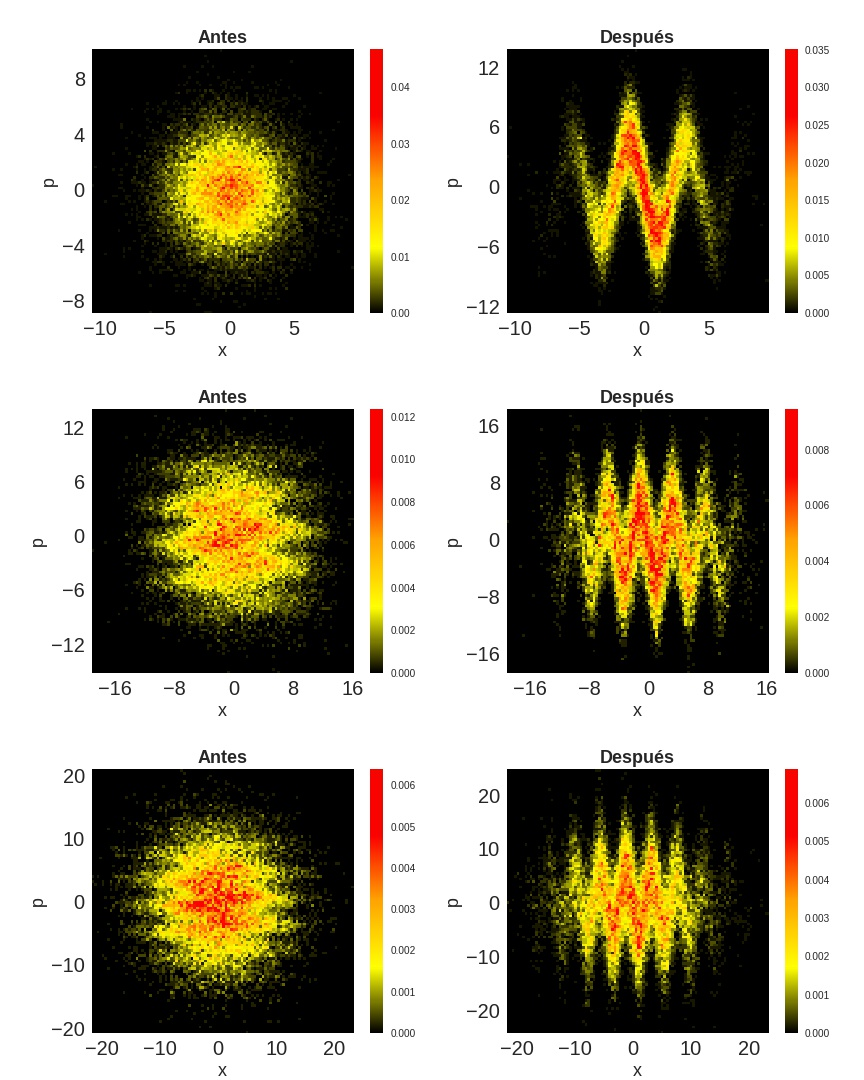
\includegraphics[width=0.85\textwidth]{last_figures/dist_functions.jpg}
	\caption{Funci\'on de distribuci\'on del sistema con $\kappa=-4.5$, $K_BT_e = 5$ y $\omega=1$, antes y despu\'es de las patadas n\'umero 1, 5 y 35 en la primera, segunda y tercera fila, respectivamente.}
\end{figure}

Las oscilaciones que aparecen en las funciones de distribuci\'on del sistema despu\'es de la patada se deben al efecto de esta, la cual depende del seno de la posici\'on $x$; durante el tiempo entre las patadas, el efecto del oscilador arm\'onico es una rotaci\'on del espacio de fase, por lo que justo antes de la siguiente patada las oscilaciones aparecen en una direcci\'on distinta. Para este caso, la rotaci\'on es de $\frac{\pi}{2}$ rad debido al par\'ametro $q=4$.


Al variar el par\'ametro de Lamb-Dicke, el \'unico efecto sobre el sistema es un reescalamiento de la funci\'on de distribuci\'on del sistema como se muestra en la figura \ref{fig.CambioEtaAjustesSeno} para los valores $\eta_{\rm LD} = 1$ y $\eta_{\rm LD} = 0.25$. Las oscilaciones en el espacio de fase antes de la patada est\'a dada por $w_o = \sqrt{2}\eta_{\rm LD}$ debido al potencial de la patada que aparece en el hamiltoniano (\ref{Hamiltoniano}) del sistema. En cambio, justo antes despu\'es de las patadas esta frecuencia ya no coincide ex\'actamente con este valor, sino que es un poco mayor, mostrado en la figura \ref{fig.FrecuenciaOscilacionesWo}.

\begin{figure}
	\centering
	\label{fig.FrecuenciaOscilacionesWo}
	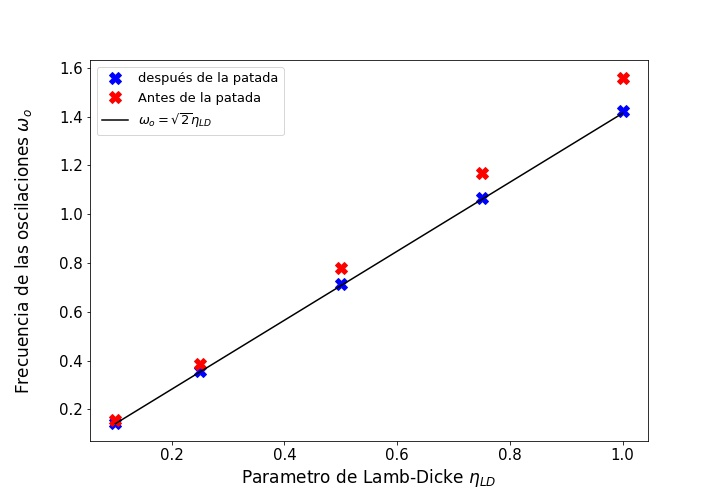
\includegraphics[width=0.7\textwidth
	]{FigsJPG/frecuencias_wk}
\end{figure}

La figura \ref{fig.CambioEtaAjustesSeno} muestra tambi\'en los ajustes a funciones sinusoide (en azul), las cuales se obtienen dividiendo $p$ y $x$ (para antes y despu\'es de la patada, respectivamente) en intervalos pequeños, realizando promedio en cada intervalo de $x$ y $p$, respectivamente, y haciendo ajustes a una funci\'on de tipo $f(x) = A\sin(\omega x + \phi)$.

\begin{figure}[h!]
	\centering
	\begin{minipage}{0.9\textwidth}
		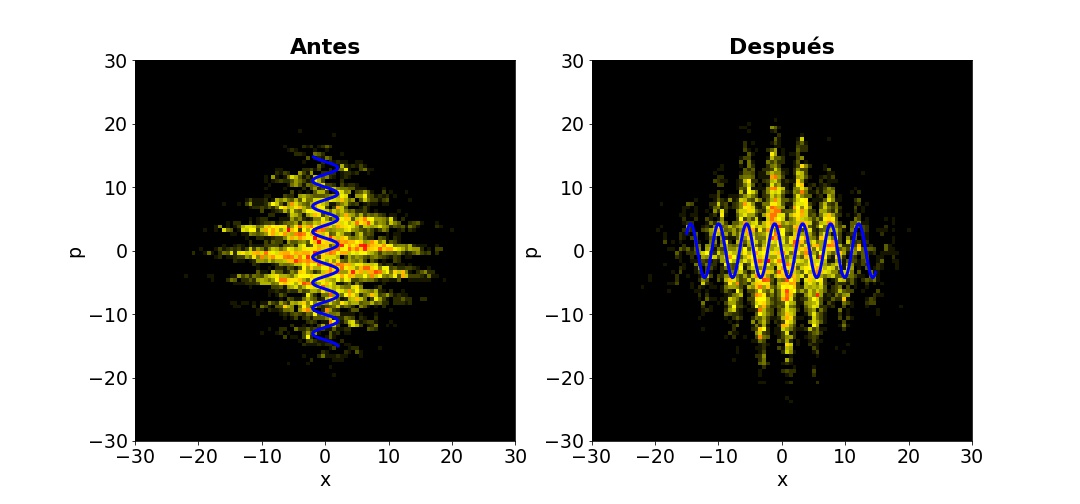
\includegraphics[width=1\textwidth]{FigsJPG/dist_function_eta_1-00}
	\end{minipage}
	\begin{minipage}{0.9\textwidth}
		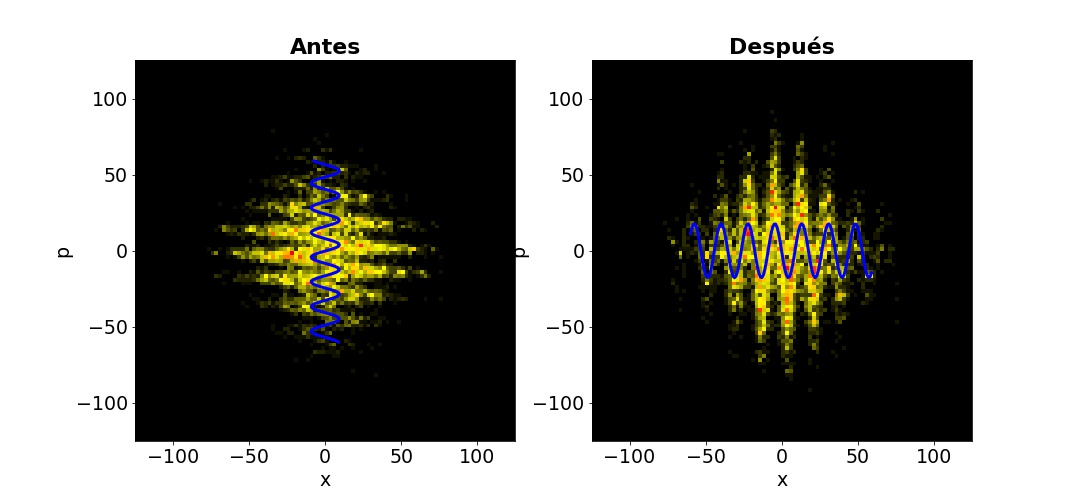
\includegraphics[width=1\textwidth]{FigsJPG/dist_function_eta_0-25}
	\end{minipage}
	\caption{Funciones de distribuci\'on antes y despu\'es de la patada 36 para el sistema con $k_BT_e=5$ usando $\eta_{\rm LD}=1$ (superior) y $\eta_{\rm LD}=0.25$ (inferior), as\'i como ajustes de las distribuciones a funciones sinusoide.}
	\label{fig.CambioEtaAjustesSeno}
\end{figure}


Para comparar las distribuciones clásicas con las funciones de Wigner publicadas en \cite{ArticuloPrado}, consideramos la función de distribución del sistema en el estado de cuasi-equilibrio del sistema, antes y después de la patada 36, para 100000 trayectorias.

La figura \ref{fig:ClasicoCuanticoPS} muestra dicha función para el sistema acoplado al reservorio a temperatura cero (superior), y las funciones de Wigner del sistema cuántico a la temperatura $k_BT_e = 5$  (inferior). En ambos casos, antes y después de la patada, podemos observar que la función de distribución del sistema clásico tiene cierta similitud con las funciones de Wigner del sistema cuántico, con las distribuciones de manera ondulatoria en las mismas direcciones y centradas en el origen, pero presentan varias diferencias, en parte debido a que la temperatura del resevorio en el sistema clásico es cero, mientras que en el caso cuántico no.

\begin{figure}
	\centering
	\hspace{0.2cm}
	\begin{minipage}{0.9\textwidth}
		\centering
		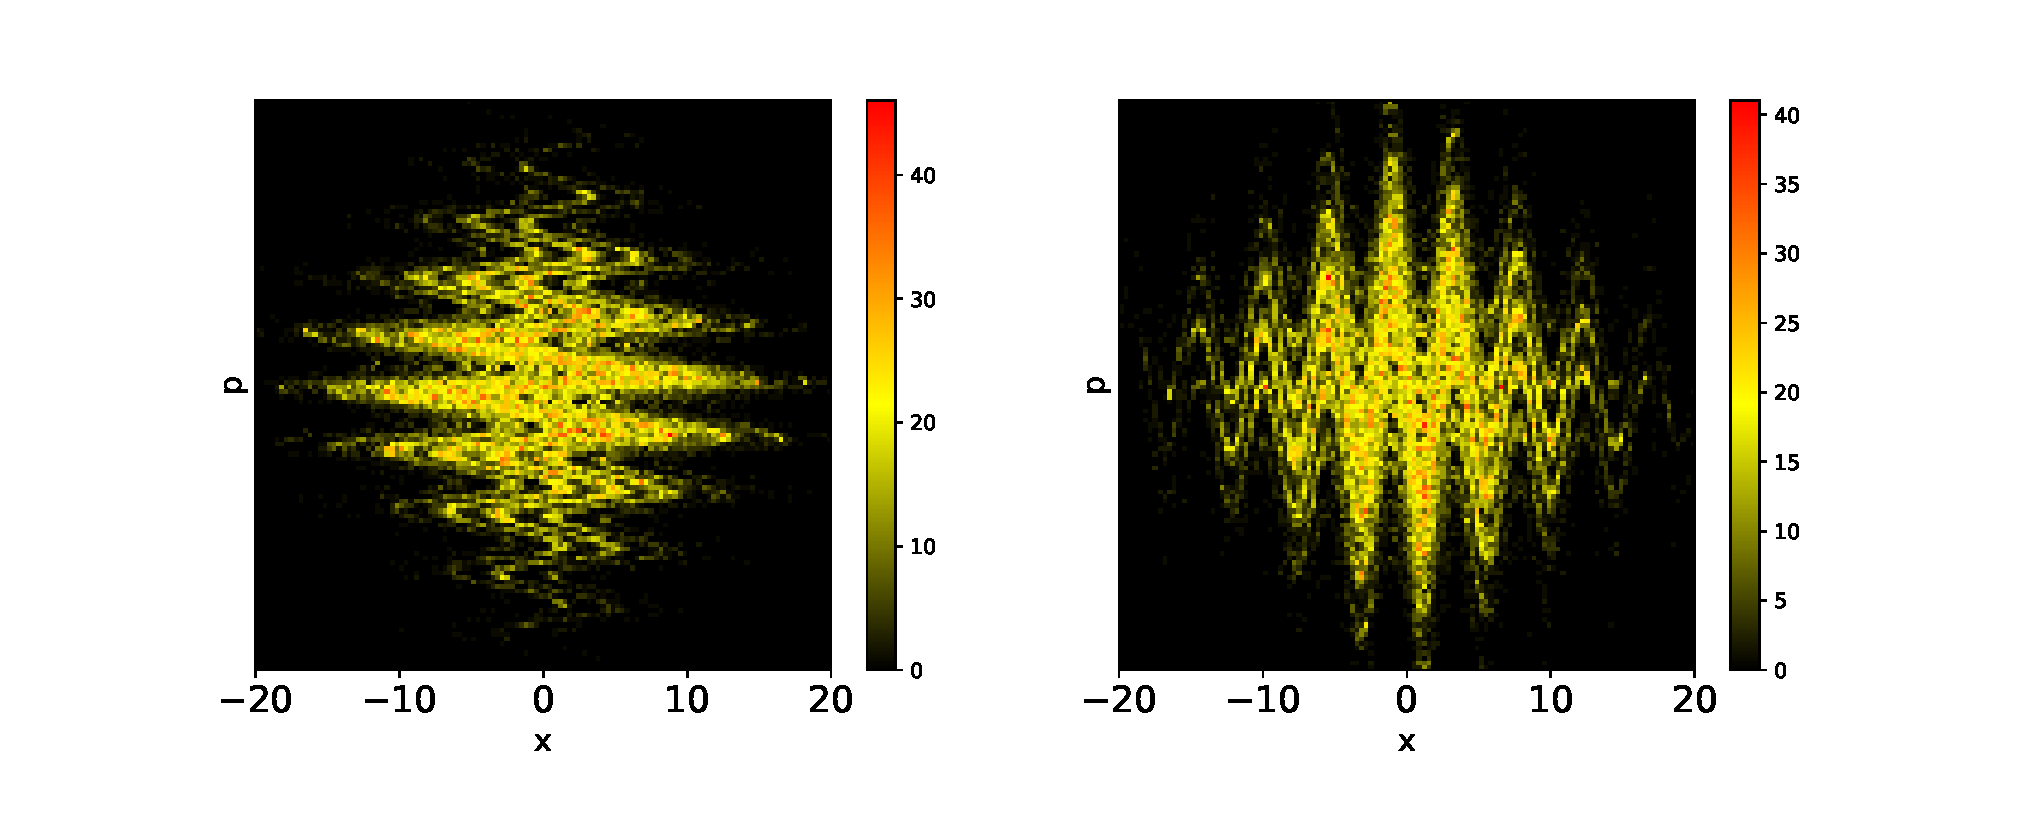
\includegraphics[width=16.1cm]{Figs/CalorMapk45T0.pdf}
		%\caption{Distribución de las partículas en el espacio de fase, antes y después de la patada 36, para $q=4$, $\beta=0.05$ y $\kappa=-4.5$.}
		
	\end{minipage}\\
	\begin{minipage}{0.45\textwidth}
		\hspace{1.2cm}
		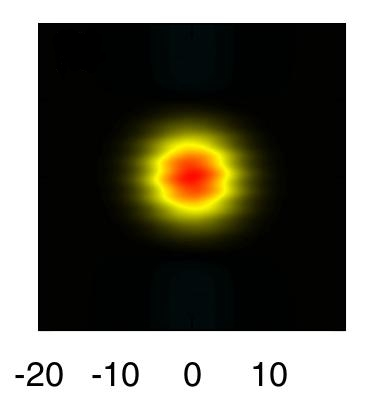
\includegraphics[width=6cm]{Figures/WignerFunctions1}
		
		%\caption{Funciones de Wigner del sistema cuántico, antes y después de la patada 36, para $q=4$, $\beta=0.05$ y $\kappa=-4.5$\cite{MPradoEtAl}.}
		
	\end{minipage}
	\begin{minipage}{0.45\textwidth}
		\hspace{0cm}
		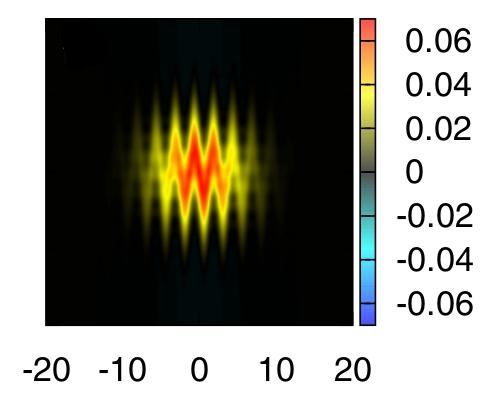
\includegraphics[width=7.99cm]{Figures/WignerFunctions2}
		
		%\caption{Funciones de Wigner del sistema cuántico, antes y después de la patada 36, para $q=4$, $\beta=0.05$ y $\kappa=-4.5$\cite{MPradoEtAl}.}
		
	\end{minipage}
	\caption{Parte superior: función de densidad del sistema clásico con la temperatura del reservorio $k_BT_e = 0$, y parte inferior: funciones de wigner del sistema cuántico con la temperatura del reservorio $k_BT_e = 5$, antes y después de la patada número 36, para $q=4$, $\beta = 0.1$ y  $\kappa=4.5$}
	
	\label{fig:ClasicoCuanticoPS}
\end{figure}


Consideramos ahora la temperatura del reservorio con $k_BT_e = 5$, el mismo valor considerado en \cite{ArticuloPrado}. La figura \ref{fig:ClasicoCuanticoPS2} muestra nuevamente las funciones de Wigner obtenidas del sistema cuántico (inferior) y la función de distribución del sistema clásico (superior), antes y después de la patada 36.

\begin{figure}[h!]
	\centering
	\hspace{0.2cm}
	\begin{minipage}{0.8\textwidth}
		\centering
		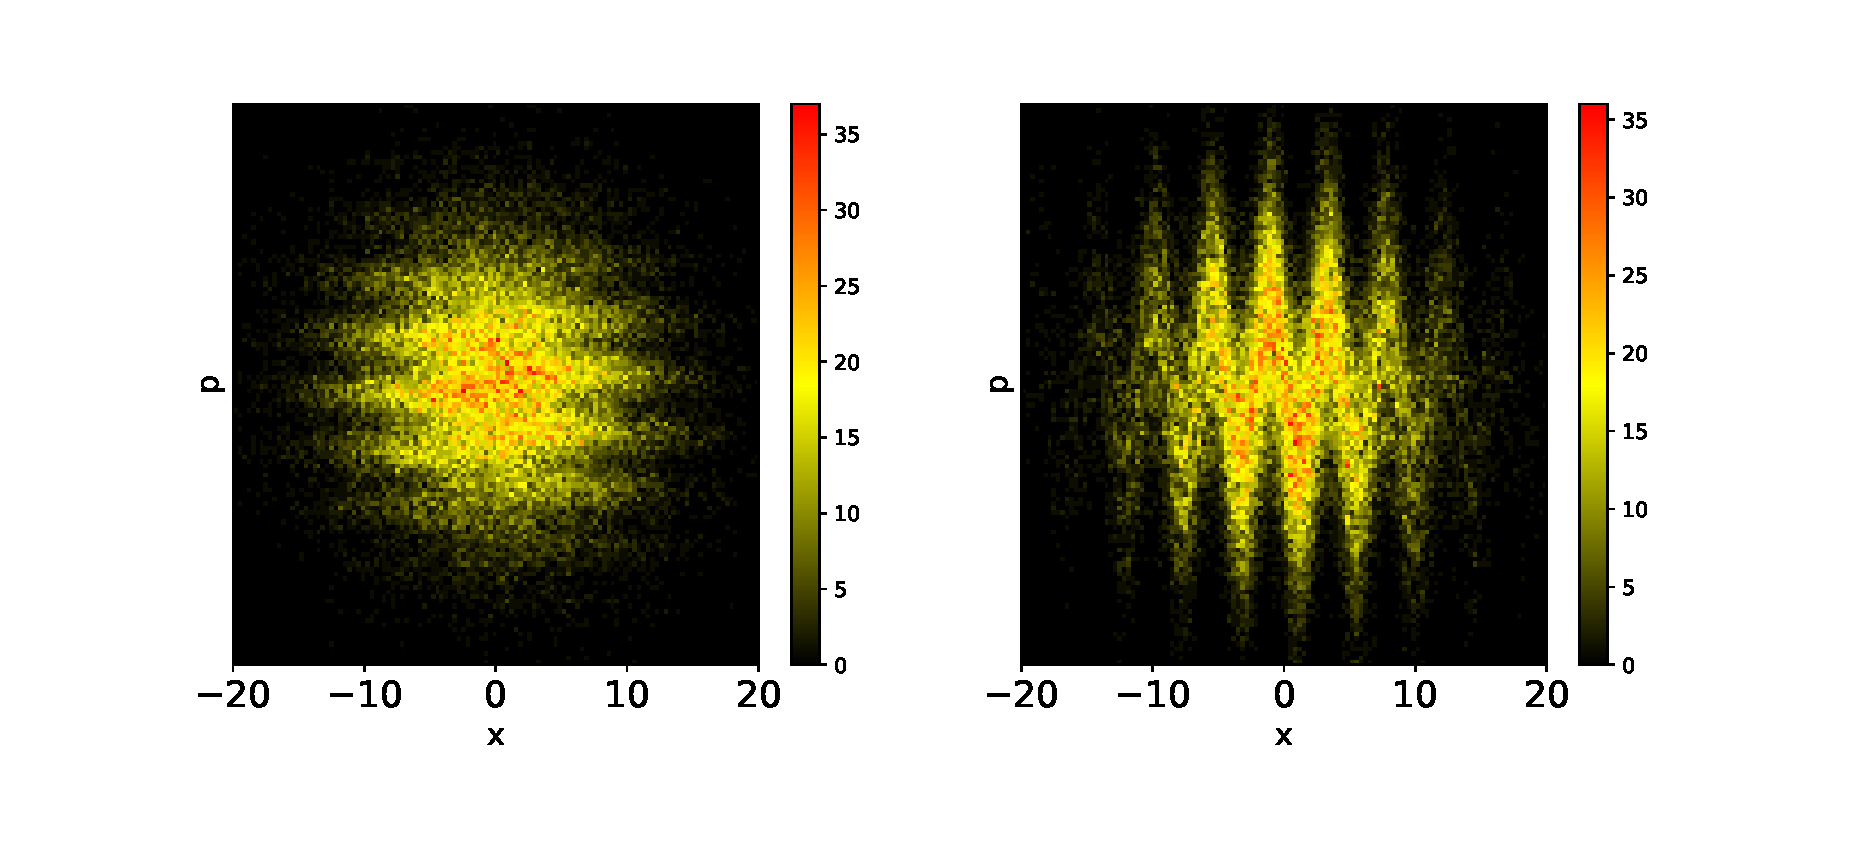
\includegraphics[width=14.5cm]{Figs/CalorMapk45T5.pdf}
		%\caption{Distribución de las partículas en el espacio de fase, antes y después de la patada 36, para $q=4$, $\beta=0.05$ y $\kappa=-4.5$.}
		
	\end{minipage}\\
	\begin{minipage}{0.34\textwidth}
		
		\hspace{0.3cm}
		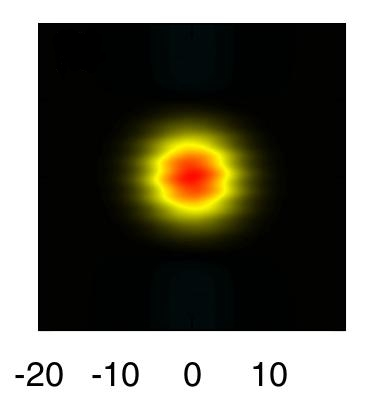
\includegraphics[width=5.35cm]{Figures/WignerFunctions1}
		
		%\caption{Funciones de Wigner del sistema cuántico, antes y después de la patada 36, para $q=4$, $\beta=0.05$ y $\kappa=-4.5$\cite{MPradoEtAl}.}
		
	\end{minipage}
	\begin{minipage}{0.34\textwidth}
		\hspace{0.2cm}
		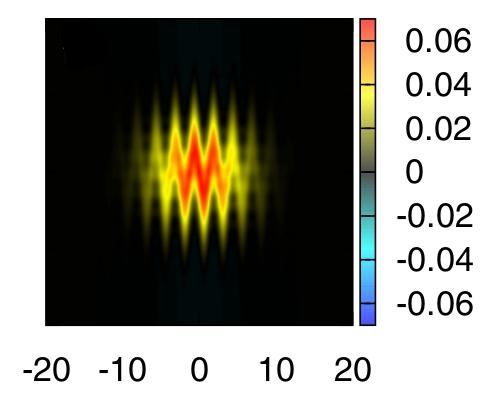
\includegraphics[width=7.2cm]{Figures/WignerFunctions2}
		
		%\caption{Funciones de Wigner del sistema cuántico, antes y después de la patada 36, para $q=4$, $\beta=0.05$ y $\kappa=-4.5$\cite{MPradoEtAl}.}
		
	\end{minipage}
	
	
	\caption{Parte superior: función de densidad del sistema clásico, y parte inferior: funciones de wigner del sistema cuántico, ambos con la temperatura del reservorio a $k_BT_e = 5$, antes y después de la patada número 36, para $q=4$, $\beta = 0.1$ y  $\kappa=4.5$}
	\label{fig:ClasicoCuanticoPS2}
	
	
\end{figure}

En este caso, al utilizar la misma temperatura que el utilizado en el caso cuántico observamos que la similitud entre los dos casos es mayor que en el caso anterior con la temperatura del reservorio en cero: nuevamente, el espacio de fase muestra una distribución semejante a una ondulación en las mismas direcciones y centrada en el origen, sin embargo existen diferencias entre ambas distribuciones, especialmente en la escala de las funciones: en el caso cuántico, los valores no nulos de las funciones de Wigner se encuentran aproximádamente en los valores de $x$ y $p$ en el rango $[-10,10]$, mientras que en el caso clásico estos mismos valores están aproximádamente en el rango $[-20,20]$

\section{Coeficientes de Fourier}


Después de un cierto número de patadas, el sistema llega a un estado de cuasi equilibrio entre la energía recibida por las patadas y la energía cedida al reservorio en forma de calor, de manera que la energía promedio antes y después de las patadas es constante, tal como sucede en el caso cuántico (figura \ref{fig:EnergiaNormal}).

\begin{figure}[h!]
	\centering
	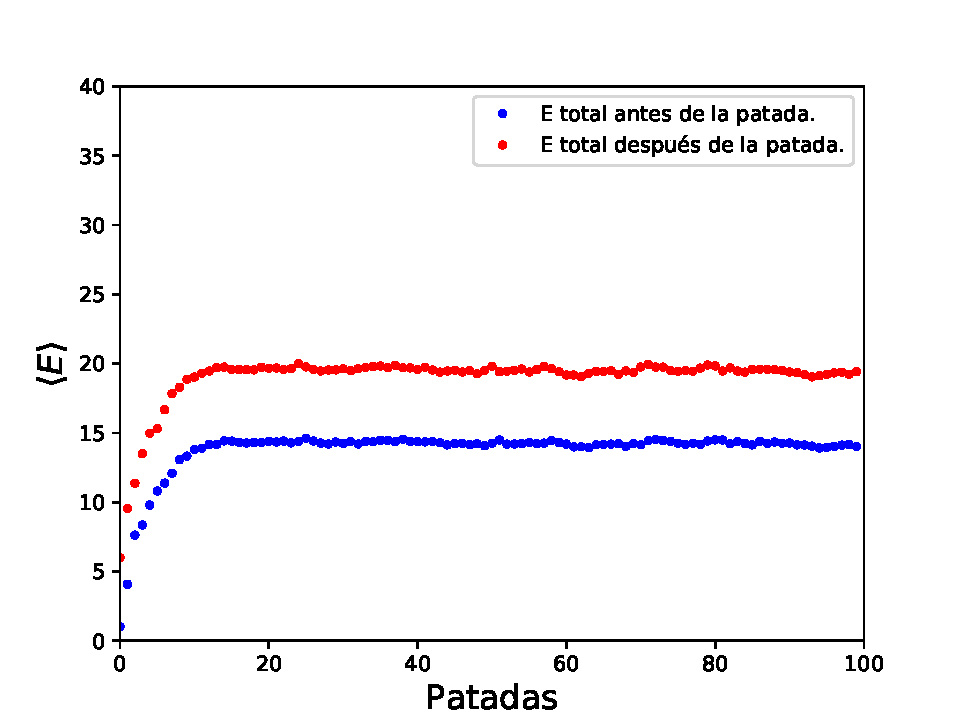
\includegraphics[width=12cm]{Figs/EvolucionEnergiak45}
	\caption{Evolución de la energía para $\kappa=4.5$ y $\beta=0.1$, con el reservorio a temperatura 0.}
	\label{fig:EnergiaNormal}
\end{figure}

La figura \ref{fig:CoeffsFourierT0} muestra los valores de los coeficientes obtenidos numéricamente con la ecuación (\ref{eq:FourierNumericalCoeffs}) para el sistema acoplado a un reservorio a temperatura 0 en estos estados, para diferentes valores de $\beta$ y $\kappa$.

\begin{figure}[h!]
	\centering
	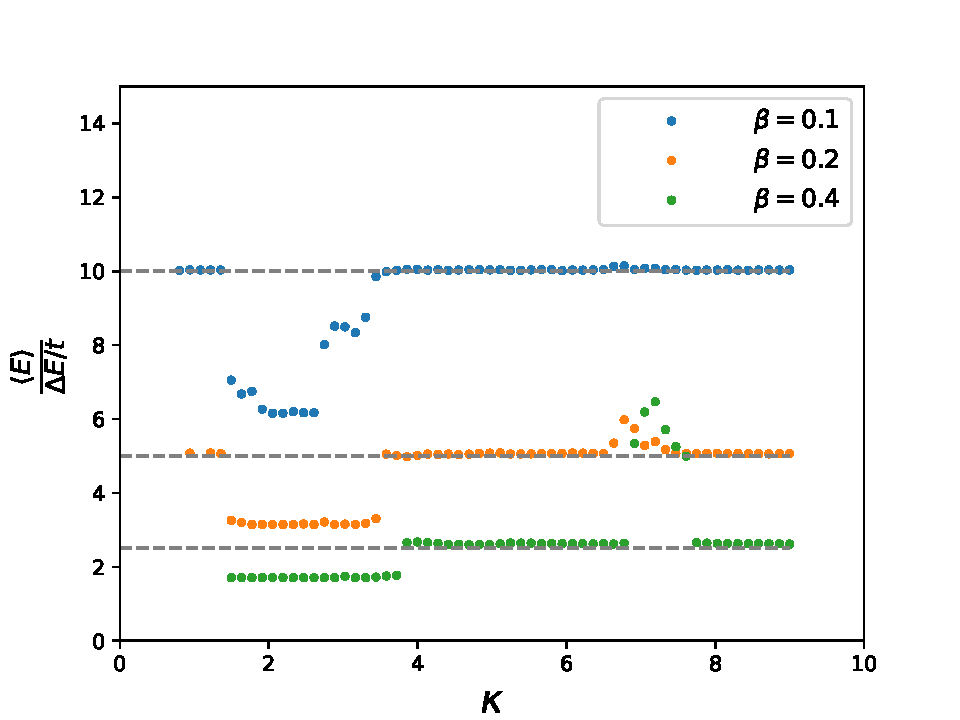
\includegraphics[width=12cm]{Figs/FourierCoeffsT0}
	\caption{Coeficientes de Fourier para diferentes valores de $\kappa$ y del coeficiente $\beta$ de acoplamiento entre el sistema y el reservorio a temperatura cero. Las líneas horizontales corresponden a las aproximaciones analíticas dadas por $\alpha=1/\beta.$}
	\label{fig:CoeffsFourierT0}
\end{figure}

En general, se observa que el sistema satisface la ley de Fourier y que los coeficientes de Fourier se ajustan a $\alpha=\frac{1}{\beta}$, igual que en el caso cuántico, excepto por tres zonas:

Cuando la fuerza de amortiguamiento es grande y las patadas pequeñas, la fuerza de amortiguamiento domina sobre el sistema y hace que este pierda toda su energía, como se muestra en la figura \ref{fig:Caso1}; para $\beta = 0.1$ todos los puntos aparecen, ya que la fuerza de amortiguamiento no es muy grande. En cambio, para $\beta = 0.2$ ya falta el valor de $\kappa$ más pequeño, mientras que al aumentar el amortiguamiento hasta $\beta = 0.4$ ya comienzan a faltar más valores, correspondientes a aproximádamente $\kappa < 1.5$.

\begin{figure}[h!]
	\centering
	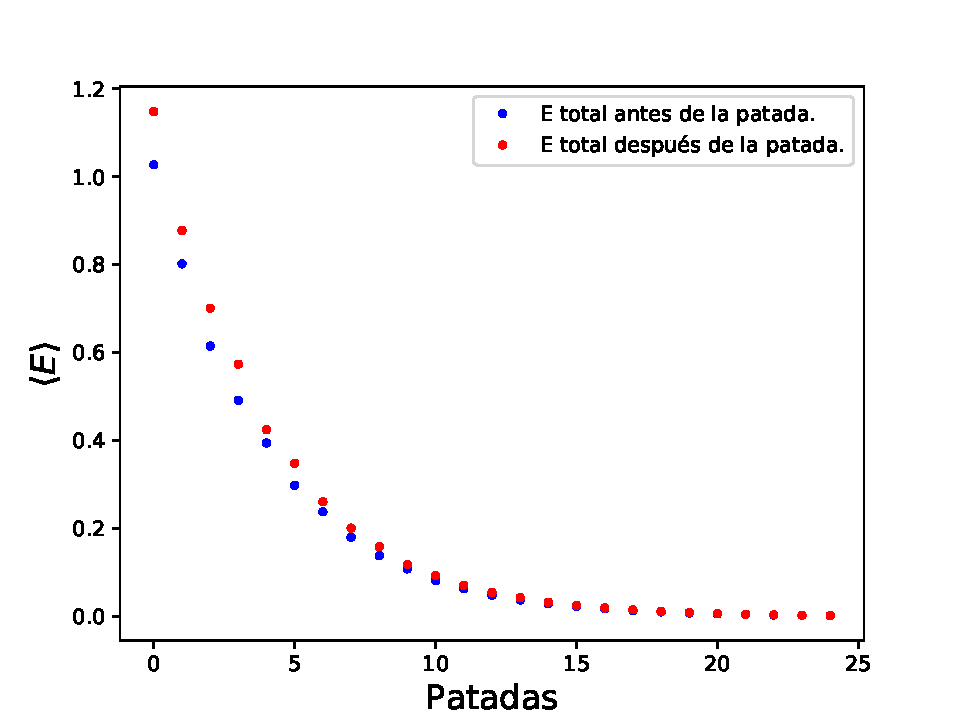
\includegraphics[width=12cm]{Figs/EnergiaCaso1}
	\caption{Evolución de la energía del sistema para $\beta=0.2$ y $\kappa=0.7$, con el reservorio a temperatura cero}
	\label{fig:Caso1}
\end{figure}

En las otras dos zonas donde los coeficientes no se ajustan a $1/\beta$, para aproximádamente $1.5<\kappa<3.5$ o $6.5<\kappa<7.6$, siendo ligeramente diferentes para cada valor de $\beta$, el sistema presenta puntos de atractores en los cuales convergen todas las trayectorias después de un cierto número de patadas, alrededor de 60 en el primer caso (figura \ref{fig:Atractores1}) y 1800 para el segundo caso (figura \ref{fig:Atractores2}). En estos casos, durante las primeras patadas el sistema aumenta su energía hasta llegar a un valor máximo, y a partir de ahí comienza a disminuir (figura \ref{fig:EnergiaAtractores}) mientras las trayectorias convergen hacia los atractores, además de que se presentan solo para los valores más grandes de la fuerza de amortiguamiento.



\begin{figure}[h!]
	\centering
	\begin{minipage}{0.32\textwidth}
		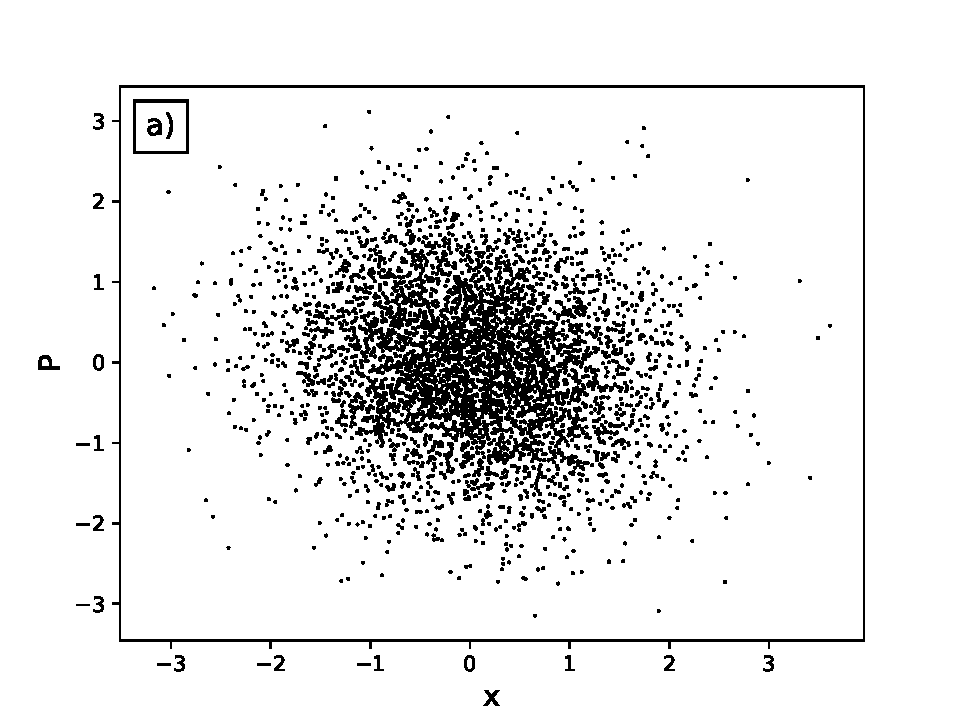
\includegraphics[width=6.5cm]{Figs/PhaseSpaceInitial}
	\end{minipage}
	\begin{minipage}{0.32\textwidth}
		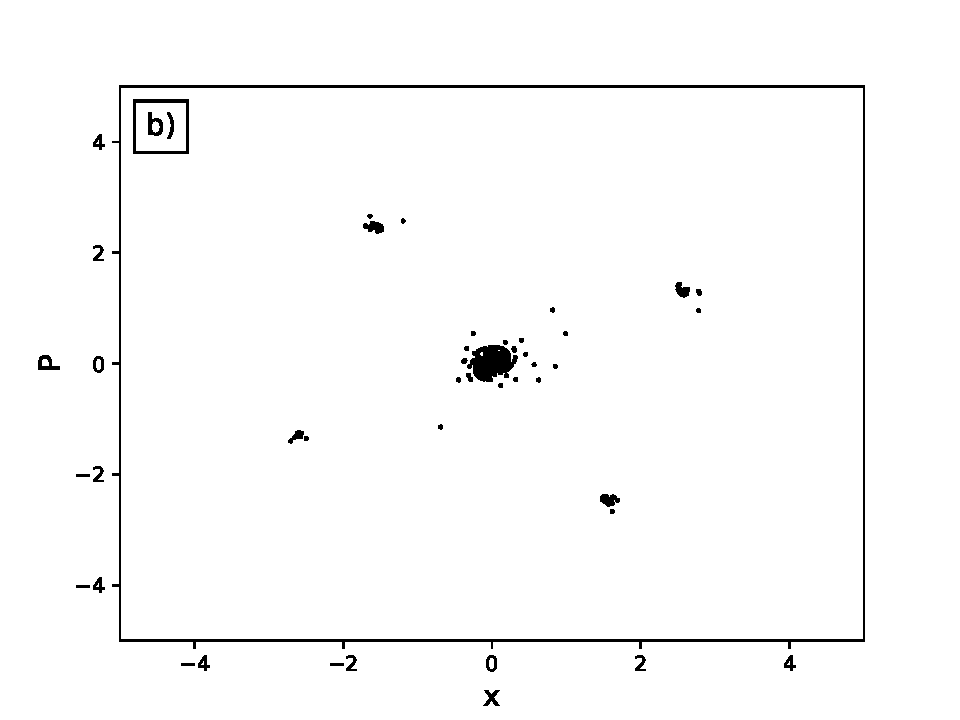
\includegraphics[width=6.5cm]{Figs/PhaseSpaceK35}
	\end{minipage}
	\begin{minipage}{0.32\textwidth}
		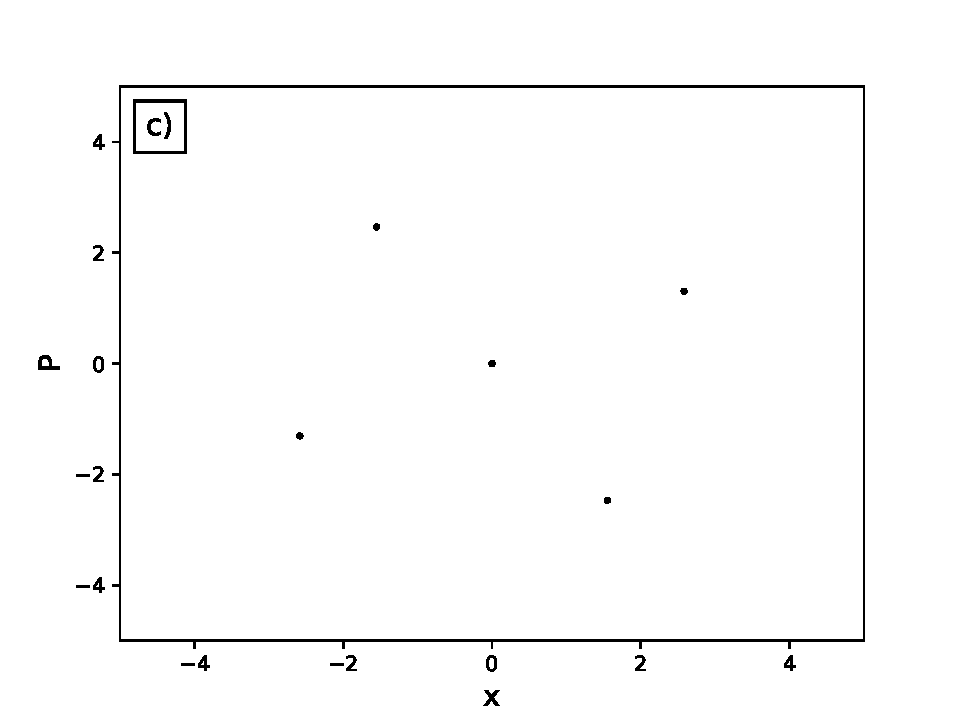
\includegraphics[width=6cm]{Figs/PhaseSpaceK100}
	\end{minipage}
	\caption{Espacio de fase del sistema a) inicial, b) después de 35 patadas y c) después de 100 patadas para $\beta=0.2$, $\kappa=7.25$, con el reservorio a temperatura 0}
	\label{fig:Atractores1}
	
\end{figure}

\begin{figure}[h!]
	\centering
	\begin{minipage}{0.32\textwidth}
		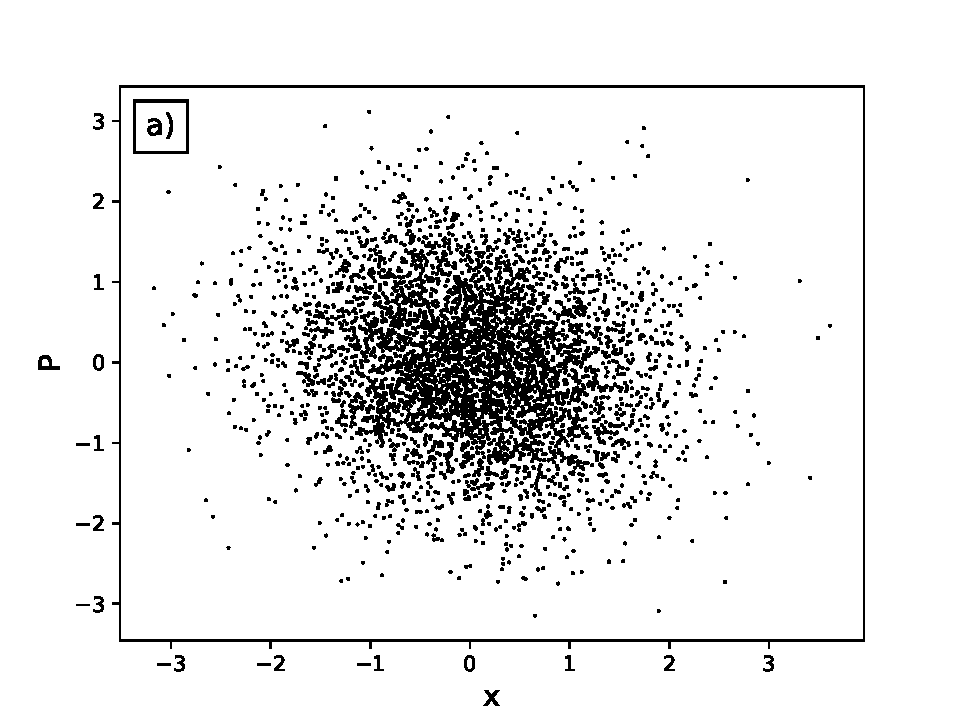
\includegraphics[width=6cm]{Figs/PhaseSpaceInitial}
	\end{minipage}
	\begin{minipage}{0.32\textwidth}
		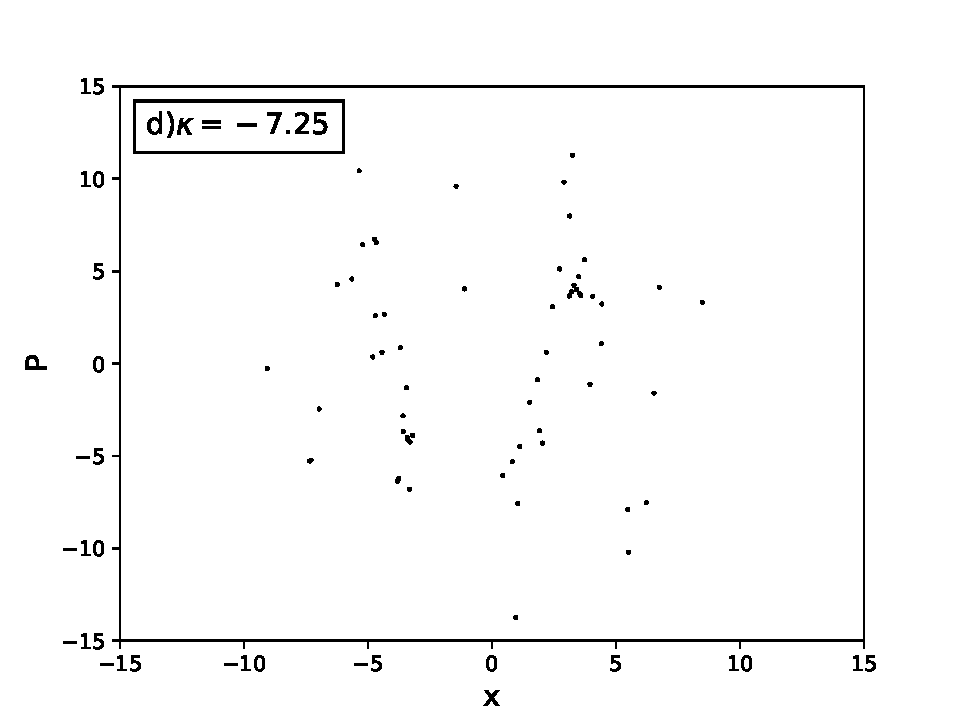
\includegraphics[width=6cm]{Figs/PhaseSpace725K1000Aft}
	\end{minipage}
	\begin{minipage}{0.32\textwidth}
		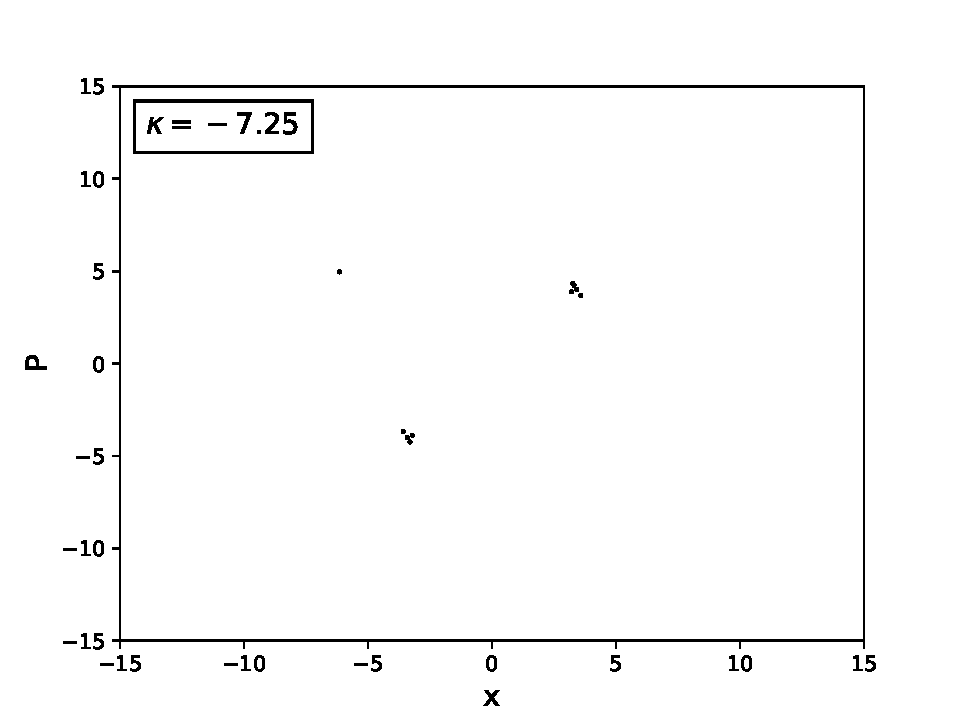
\includegraphics[width=6cm]{Figs/Atractoresk725}
	\end{minipage}
	\caption{Espacio de fase del sistema a) inicial, b) después de 1000 patadas y c) después de 1500 patadas para $\beta=0.2$, $\kappa=0.7$, con el reservorio a temperatura 0}
	\label{fig:Atractores2}
	
\end{figure}

\begin{figure}[h!]
	\centering
	\begin{minipage}{0.45\textwidth}
		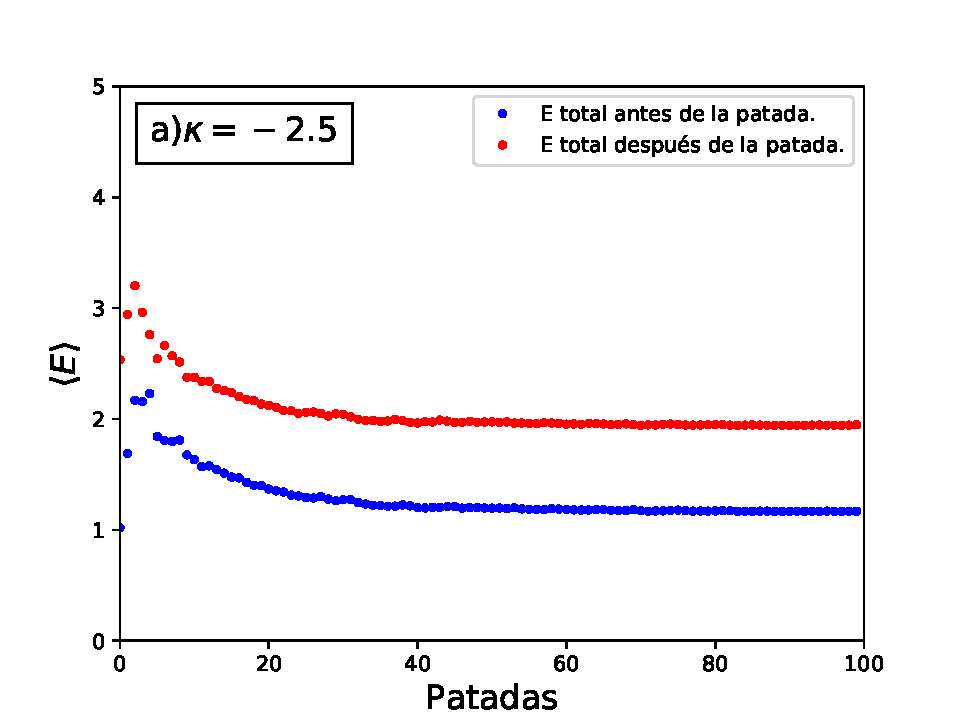
\includegraphics[width=8.5cm]{Figs/EnergiaK25}
	\end{minipage}
	\begin{minipage}{0.45\textwidth}
		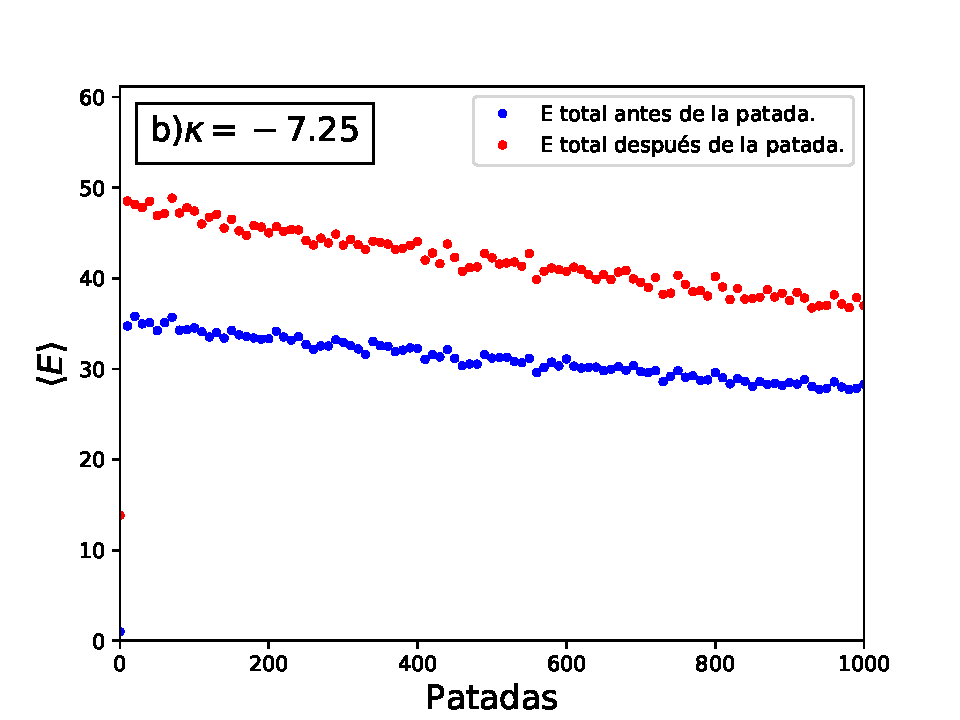
\includegraphics[width=8.5cm]{Figs/EnergiaK725}
	\end{minipage}
	\caption{Evolución de la energía para los valores de a)$\kappa=2.5$ y  b)$\kappa=7.25$, con $\beta=0.2$ y el reservorio a temperatura 0.}
	\label{fig:EnergiaAtractores}
\end{figure}


La figura \ref{fig:CoeffsFourierT5} muestra los coeficientes de Fourier obtenidas para valores diferentes de $\beta$ y $\kappa$, con la temperatura del reservorio en $k_BT_e = 0.1$ y $k_BT_e = 5$.

\begin{figure}[h!]
	\centering
	\begin{minipage}{0.45\textwidth}
		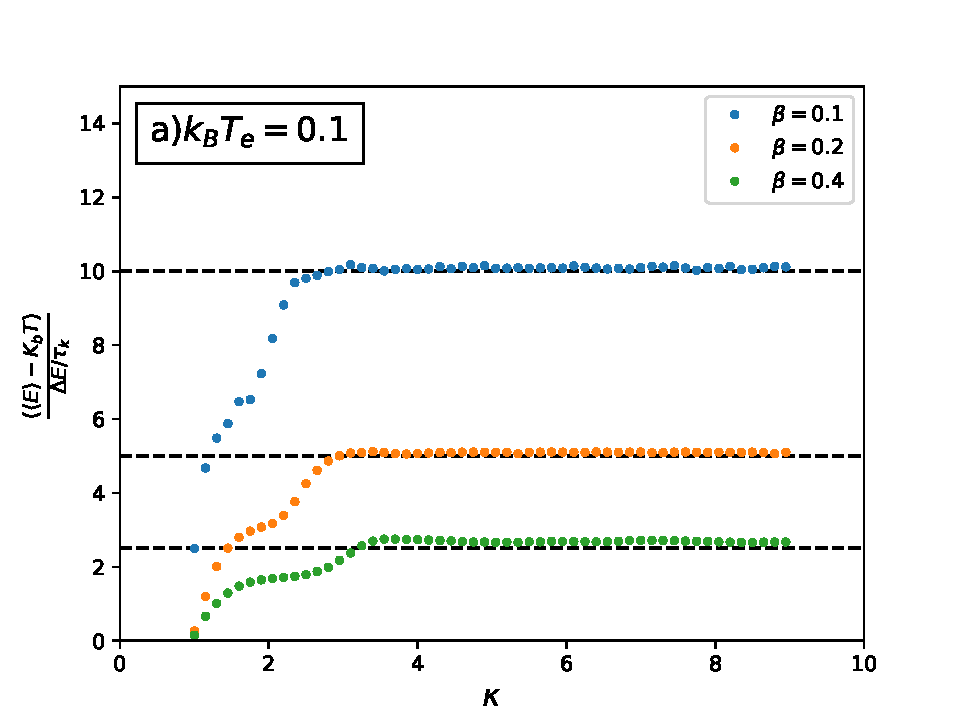
\includegraphics[width=8.5cm]{Figs/FourierCoeffsT01}
	\end{minipage}
	\begin{minipage}{0.45\textwidth}
		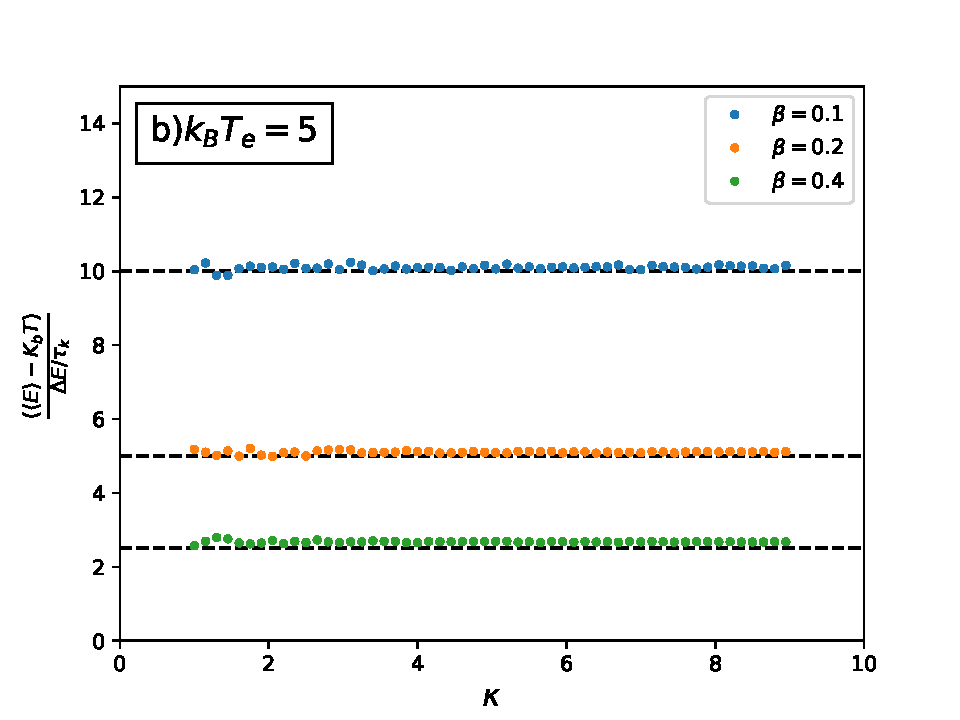
\includegraphics[width=8.5cm]{Figs/FourierCoeffsT5}
	\end{minipage}
	\caption{Coeficientes de la ley de Fourier para diferentes valores de $\beta$ y $\kappa$, agregando una temperatura definida para el reservorio, $k_BT_e$. Las líneas horizontales corresponden a las predicciónes analíticas dadas por $\alpha=1/\beta.$}
	\label{fig:CoeffsFourierT5}
\end{figure}

Al utilizar una temperatura para el reservorio suficientemente grande, estas zonas desaparecen y el sistema satisface la ley de Fourier para todos los valores de $\beta$ y $\kappa$ (figura\ref{fig:CoeffsFourierT5}). Debido a la temperatura del entorno, actúa una fuerza aleatoria sobre las partículas que no depende de su estado, lo que evita que el sistema pierda toda su energía o converja a los atractores. Como se puede ver en la figura \ref{fig:CoeffsFourierT5}a, los atractores alrededor de $\kappa = 7.25$ desaparecen con temperaturas muy pequeñas, mientras que los de la otra zona comienzan a desaparecer primero para los valores mayores de $\kappa$ y luego hacia los menores a medida que se va incrementando esta temperatura.




\section{Comparación con la distribución de Boltzmann}

La figura \ref{fig:ComparacionBoltzmann} muestra el histograma normalizado de la función de distribución, y el porcentaje del error absoluto con respecto a la distribución de Boltzmann en cada celda (inferior), antes y después de la patada 40, una vez que el sistema se encuentra en el cuasi-equilibrio, considerando el sistema con 75000 partículas.

\begin{figure}[h!]
	
	\hspace{-0.5cm}
	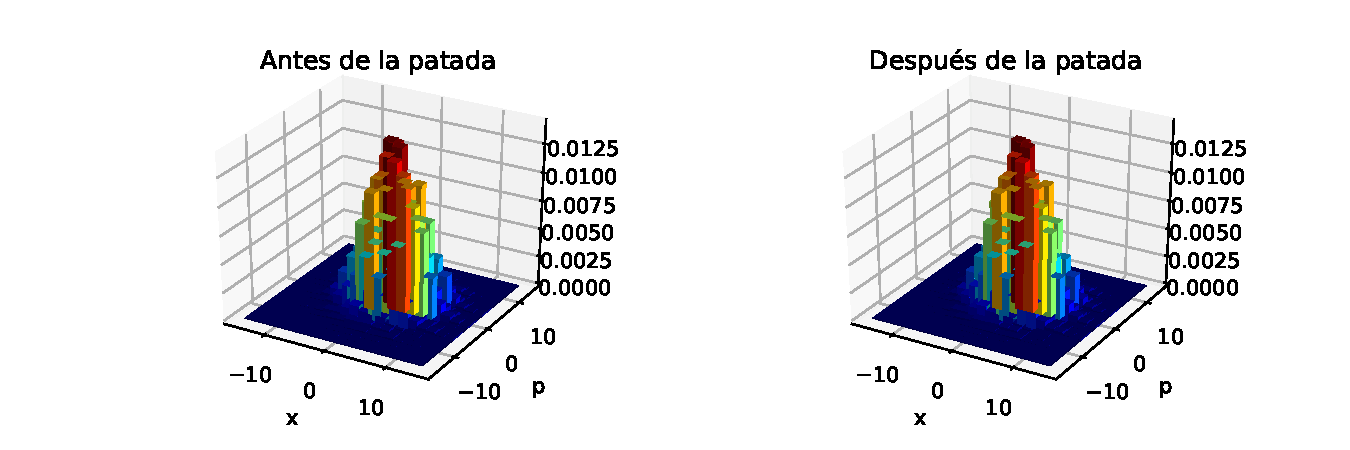
\includegraphics[width=18cm]{Figs/DistribucionesK20T5Kick40}\\
	
	
	%\vspace{-0.5cm}
	\hspace{-0.2cm}
	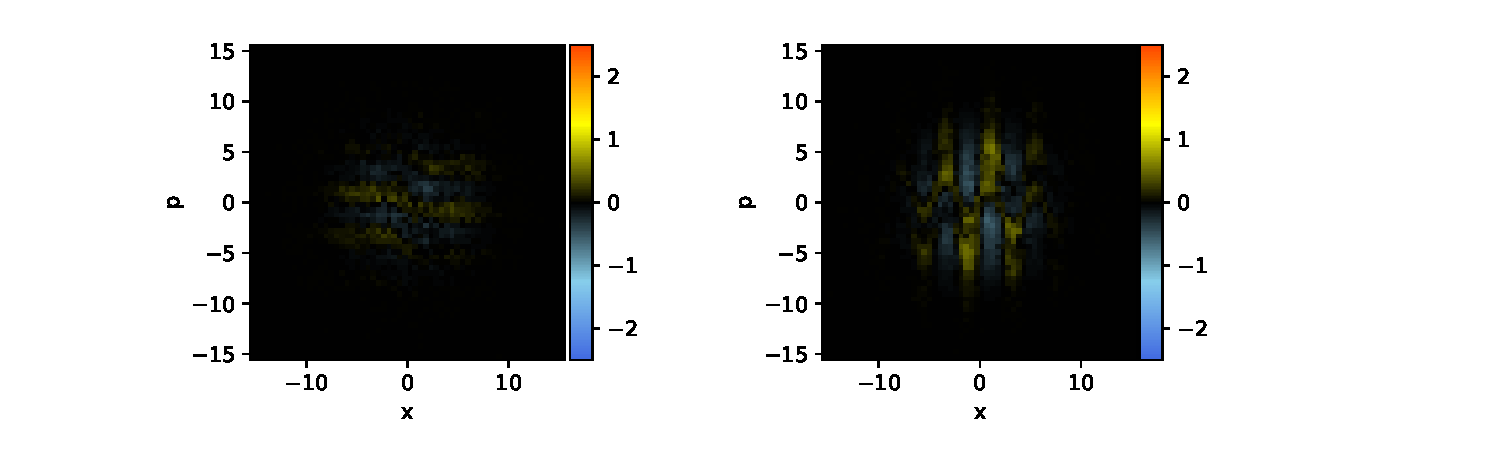
\includegraphics[width=20cm]{Figs/DiferenciasK20T5Kick40}
	%\vspace{-0.5cm}
	\caption{Histograma de la función de distribución del sistema durante la patada 40 (superior), y el porcentaje de diferencia con la distribución de Boltzmann en cada celda (inferior), para $\kappa=2.0$, $\beta=0.1$ y el reservorio con $k_BT_e = 5$.}
	\label{fig:ComparacionBoltzmann}
\end{figure}


En ambos casos, antes y después de la patada, vemos que la diferencia entre las distribuciones no sobrepasa el 1\% en los valores máximos, cuando el sistema se encuentra en el cuasi-equilibrio con el reservorio,  siendo mayores justo después de las patadas.

La tabla \ref{tab:ErroresPorcentaje} muestra el porcentaje del error absoluto entre la función de distribución del sistema y la distribución de Boltzmann para distintos valores de $\kappa$ y el valor de $k_BT_e$ del reservorio dado por la ecuación (\ref{eq:ErrorTotal}), para el momento justo antes después y justo después de la patada 40, respectivamente, cuando el sistema se encuentra en el cuasi-equilibrio. Para los mismos casos, se muestra la divergencia de Kullback-Leibler en la tabla \ref{tab:KL}, para antes y después de la patada 40.

\definecolor{babyblueeyes}{rgb}{0.63, 0.79, 0.95}


\renewcommand{\tablename}{Tabla}

\begin{table}[h!]
	\centering
	\begin{tabular}{|>{\columncolor{blue!10}}c||c|c||c|c||c|c||c|c||c|c||}\hline
		\rowcolor{blue!10}  \backslashbox{$\kappa$}{$k_BT_e$}
		& \multicolumn{2}{|c||}{\textbf{5} (\%)} & \multicolumn{2}{|c||}{\textbf{10} (\%)}  & \multicolumn{2}{|c||}{\textbf{15} (\%)} & \multicolumn{2}{|c||}{\textbf{20} (\%)}  & \multicolumn{2}{|c||}{\textbf{25} (\%)}  \\ \hline\hline
		-2.0 & 8.2 & 17.2  & 4.95 &  13.6  & 4.15  & 11.5  & 3.65 & 10.3  & 4.1   & 9.5  \\ \hline
		-4.0 & 9.2 & 19.4  & 5.65 &  16.7  & 4.45  & 14.7  & 4.5  & 14.7  & 4.45  & 14.3  \\ \hline
		-6.0 & 8.9 & 18.6  & 5.3  &  18.7  & 5.15  & 16.5  & 5.0  & 15.9  & 4.45  & 15.3   \\ \hline
		-8.0 & 8.8 & 17.7  & 6.2  &  17.3  & 5.45  & 15.6  & 4.85 & 15.5  & 4.75  & 14.9   \\ \hline
		
	\end{tabular}
	\caption{Porcentaje del error absoluto de la función de distribución del oscilador armónico pateado con respecto a la distribución de Boltzmann del oscilador armónico, antes y después de la patada 40.}
	\label{tab:ErroresPorcentaje}
\end{table} 

\begin{table}[h!]
	\begin{tabular}{|>{\columncolor{blue!10}}c||c|c||c|c||c|c||c|c||c|c||}\hline
		
		\rowcolor{blue!10}  \backslashbox{$\kappa$}{$k_BT_e$}
		& \multicolumn{2}{|c||}{5} & \multicolumn{2}{|c||}{10}  & \multicolumn{2}{|c||}{15} & \multicolumn{2}{|c||}{20}  & \multicolumn{2}{|c||}{25}  \\ \hline
		-2.0 & 0.038&0.116 &0.023 &0.079 &0.019 & 0.064 & 0.021 &0.055 &0.017 & 0.043 \\ \hline
		
		-4.0 &0.043 &0.141 &0.023 &0.114 &0.0200 &0.101 &0.0193 & 0.089 &0.019 & 0.082 \\ \hline
		
		-6.0 &0.042 &0.137 &0.023 & 0.120&0.0240 &0.120 & 0.024 & 0.109 &0.023 & 0.103 \\ \hline
		
		-8.0 &0.036 &0.112 &0.025 &0.109 & 0.022 &0.098 & 0.023 & 0.100 &0.022 & 0.092 \\ \hline
		
	\end{tabular}
	\caption{Divergencia de Kullback-Leibler del oscilador armónico pateado con respecto al oscilador armónico antes y después de la patada 40. }
	\label{tab:KL}
	
\end{table} 

	
	\begin{thebibliography}{99}
		
		\bibitem{1991ProblemChaos} \fontsize{0.35cm}{0.5cm}\selectfont{Berman, G. P., Rubaev, V. Y., \& Zaslavsky, G. M. (1991). ``The problem of quantum chaos in a kicked harmonic oscillator. \textit{Nonlinearity}, 4(2), 543.}
		
		\bibitem{2019dynamics} \fontsize{0.35cm}{0.5cm}\selectfont{Tuwankotta, J. M., \& Ihsan, A. F. (2019). ``On the dynamics of a kicked harmonic oscillator'' \textit{International Journal of Dynamics and Control}, 7(3), 857-865}
		
		\bibitem{2008StabilityChaos} \fontsize{0.35cm}{0.5cm}\selectfont{Kells, G. A., Twamley, J., \& Heffernan, D. M. (2008) ``Stability analysis of the kicked harmonic oscillator's accelerator modes. \textit{Chaos, Solitons \& Fractals}, 36(3), 772-780}
		
		\bibitem{2012Experimental} \fontsize{0.35cm}{0.5cm}\selectfont{Lemos, G. B., Gomes, R., Walborn, S., Ribeiro, S. y Fabricio T., ``Experimental observation of quantum chaos in a beam of light''\textit{Nature Communications}, Vol. 3, No. 1, p. 01-07, 2012.}
		
		\bibitem{2017Prado} \fontsize{0.35cm}{0.5cm}\selectfont{Reynoso, M. P., Vázquez, P. L., \& Gorin, T. (2017). ``Quantum kicked harmonic oscillator in contact with a heat bath''. \textit{Physical Review A}, 95(2), 022118.}
		
		\bibitem{2004Transition} \fontsize{0.35cm}{0.5cm} \selectfont{Carvalho, A. R. R., de Matos Filho, R. L., \& Davidovich, L. (2004). ``Environmental effects in the quantum-classical transition for the delta-kicked harmonic oscillator''. \textit{Physical Review E}, 70(2), 026211.}
		
		\bibitem{2016Entanglement} \fontsize{0.35cm}{0.5cm} \selectfont{Arrais, E. G., Sales, J. S., \& de Almeida, N. G. (2016). ``Entanglement dynamics for a conditionally kicked harmonic oscillator''. \textit{Journal of Physics B: Atomic, Molecular and Optical Physics}, 49(16), 165501.
		}	
		
		\bibitem{1998LangevinEquation} \fontsize{0.35cm}{0.5cm} \selectfont{Sekimoto, K. (1998). ``Langevin equation and thermodynamics''. \textit{Progress of Theoretical Physics Supplement}, 130, 17-27}
		
		\bibitem{PradoTesis} \fontsize{0.35cm}{0.5cm}\selectfont{Prado Reynoso, M. A. (2016), ``Dinámica en el espacio de fase del oscilador armónico pateado acoplado a un reservorio térmico'' {Tesis de maestría, Universidad de Guadalajara}, 2016.}
		
		
		\bibitem{CursoFisEstadistica} \fontsize{0.35cm}{0.5cm}\selectfont{Ortin Rull, J. y Sancho Herrero J. M.(2006), ``Curso de física estadística'', \emph{}.}
		\bibitem{ModernTermo} \fontsize{0.35cm}{0.5cm}\selectfont{Helrich, S. C. (2011), ``Modern Thermodynamics with Statistical Mechanics'', Springer.}
		
		\bibitem{Energy} \fontsize{0.35cm}{0.5cm}\selectfont{Gilchrist, A. (2017), ``\emph{Energy in a Damped Harmonic Oscillator}'', {http://www.entropy.energy/scholar/node/damped-harmonic-oscillator-energy}, visitado el 24-09-2019.}
		
		\bibitem{ArticuloPrado} \fontsize{0.35cm}{0.5cm}\selectfont{Prado Reynoso, M. Á., López Vázquez, P. C., y Gorin, T., ``Quantum kicked harmonic oscillator in contact with a heat bath''\textit{Physical Review A}, Vol. 95, No. 2, p. 01-09, 2017.} 
	
		
	\end{thebibliography}
\end{document}